\documentclass[10pt]{beamer}
\usetheme[
%%% options passed to the outer theme
%    hidetitle,           % hide the (short) title in the sidebar
%    hideauthor,          % hide the (short) author in the sidebar
%    hideinstitute,       % hide the (short) institute in the bottom of the sidebar
%    shownavsym,          % show the navigation symbols
%    width=2cm,           % width of the sidebar (default is 2 cm)
%    hideothersubsections,% hide all subsections but the subsections in the current section
%    hideallsubsections,  % hide all subsections
    left               % right of left position of sidebar (default is right)
%%% options passed to the color theme
%    lightheaderbg,       % use a light header background
  ]{AAUsidebar}

% If you want to change the colors of the various elements in the theme, edit and uncomment the following lines
% Change the bar and sidebar colors:
%\setbeamercolor{AAUsidebar}{fg=red!20,bg=red}
%\setbeamercolor{sidebar}{bg=red!20}
% Change the color of the structural elements:
%\setbeamercolor{structure}{fg=red}
% Change the frame title text color:
%\setbeamercolor{frametitle}{fg=blue}
% Change the normal text color background:
%\setbeamercolor{normal text}{bg=gray!10}
% ... and you can of course change a lot more - see the beamer user manual.

\usepackage{skull}
\usepackage[utf8]{inputenc}
\usepackage[english]{babel}
\usepackage[T1]{fontenc}
% Or whatever. Note that the encoding and the font should match. If T1
% does not look nice, try deleting the line with the fontenc.
\usepackage{graphicx}
\usepackage{xcolor}
\usepackage{colortbl}
\usepackage{helvet}
\usepackage{gensymb}
\usepackage{multicol}
\usepackage{booktabs}
\usepackage{pdfpages}
\usepackage{pgfpages}

%% Uncomment the following 2 for handout with notes

%\usepackage{handoutWithNotes}
%\pgfpagesuselayout{3 on 1 with notes}[a4paper,border shrink=5mm]

% colored hyperlinks
\newcommand{\chref}[2]{%
  \href{#1}{{\usebeamercolor[bg]{AAUsidebar}#2}}%
}

\title[]% optional, use only with long paper titles
{\textit{CORPS}}

\subtitle{- Cell Operating Robot Production System -}  % could also be a conference name

\date{\today}

\author[rob1B217] % optional, use only with lots of authors
{
  rob2B374\\
  \href{mailto:rob2b374@student.aau.dk}{{\tt rob2b374@student.aau.dk}}
}
% - Give the names in the same order as they appear in the paper.
% - Use the \inst{?} command only if the authors have different
%   affiliation. See the beamer manual for an example

\institute[
%  {\includegraphics[scale=0.2]{aau_segl}}\\ %insert a company, department or university logo
  Faculty of Engineering and Science\\
  Aalborg University\\
  Denmark
] % optional - is placed in the bottom of the sidebar on every slide
{% is placed on the title page
  Faculty of Engineering and Science\\
  Aalborg University\\
  Denmark
  
  %there must be an empty line above this line - otherwise some unwanted space is added between the university and the country (I do not know why;( )
}


% specify a logo on the titlepage (you can specify additional logos an include them in 
% institute command below
\pgfdeclareimage[height=1.5cm]{titlepagelogo}{AAUgraphics/aau_logo_new} % placed on the title page
%\pgfdeclareimage[height=1.5cm]{titlepagelogo2}{graphics/aau_logo_new} % placed on the title page
\titlegraphic{% is placed on the bottom of the title page
  \pgfuseimage{titlepagelogo}
%  \hspace{1cm}\pgfuseimage{titlepagelogo2}
}



\begin{document}
% the titlepage
{\aauwavesbg%
\begin{frame}[plain,noframenumbering] % the plain option removes the sidebar and header from the title page
  \titlepage 
\end{frame}}
%%%%%%%%%%%%%%%%

% TOC
\begin{frame}{Agenda}{}
\begin{multicols}{2}
  \tableofcontents
\end{multicols}
\end{frame}
%%%%%%%%%%%%%%%%
\phantomsection
\section{Introduction}

\begin{frame}{Introduction}{Rebecca Malihi}


\begin{center}
What could be a feasible way for \textit{Grundfos} to integrate industrial manipulators in the welding process of an impeller?
\end{center}

% \begin{columns}
% \column{0.40\textwidth}


% \column{0.55\textwidth}



% \end{columns}
\end{frame}
\phantomsection
\section{Problem Analysis}
\subsection{Grunfos}
\begin{frame}

\end{frame}






\subsection{Stakeholders}
\begin{frame}

\end{frame}




\subsection{Pums and Impellers}
\begin{frame}

\end{frame}


\subsection{Welding}
\begin{frame}

\end{frame}










\subsection{Industrial Manipulators}
\begin{frame}{Industrial Manipulators}{Andrej Orsula}
\centering
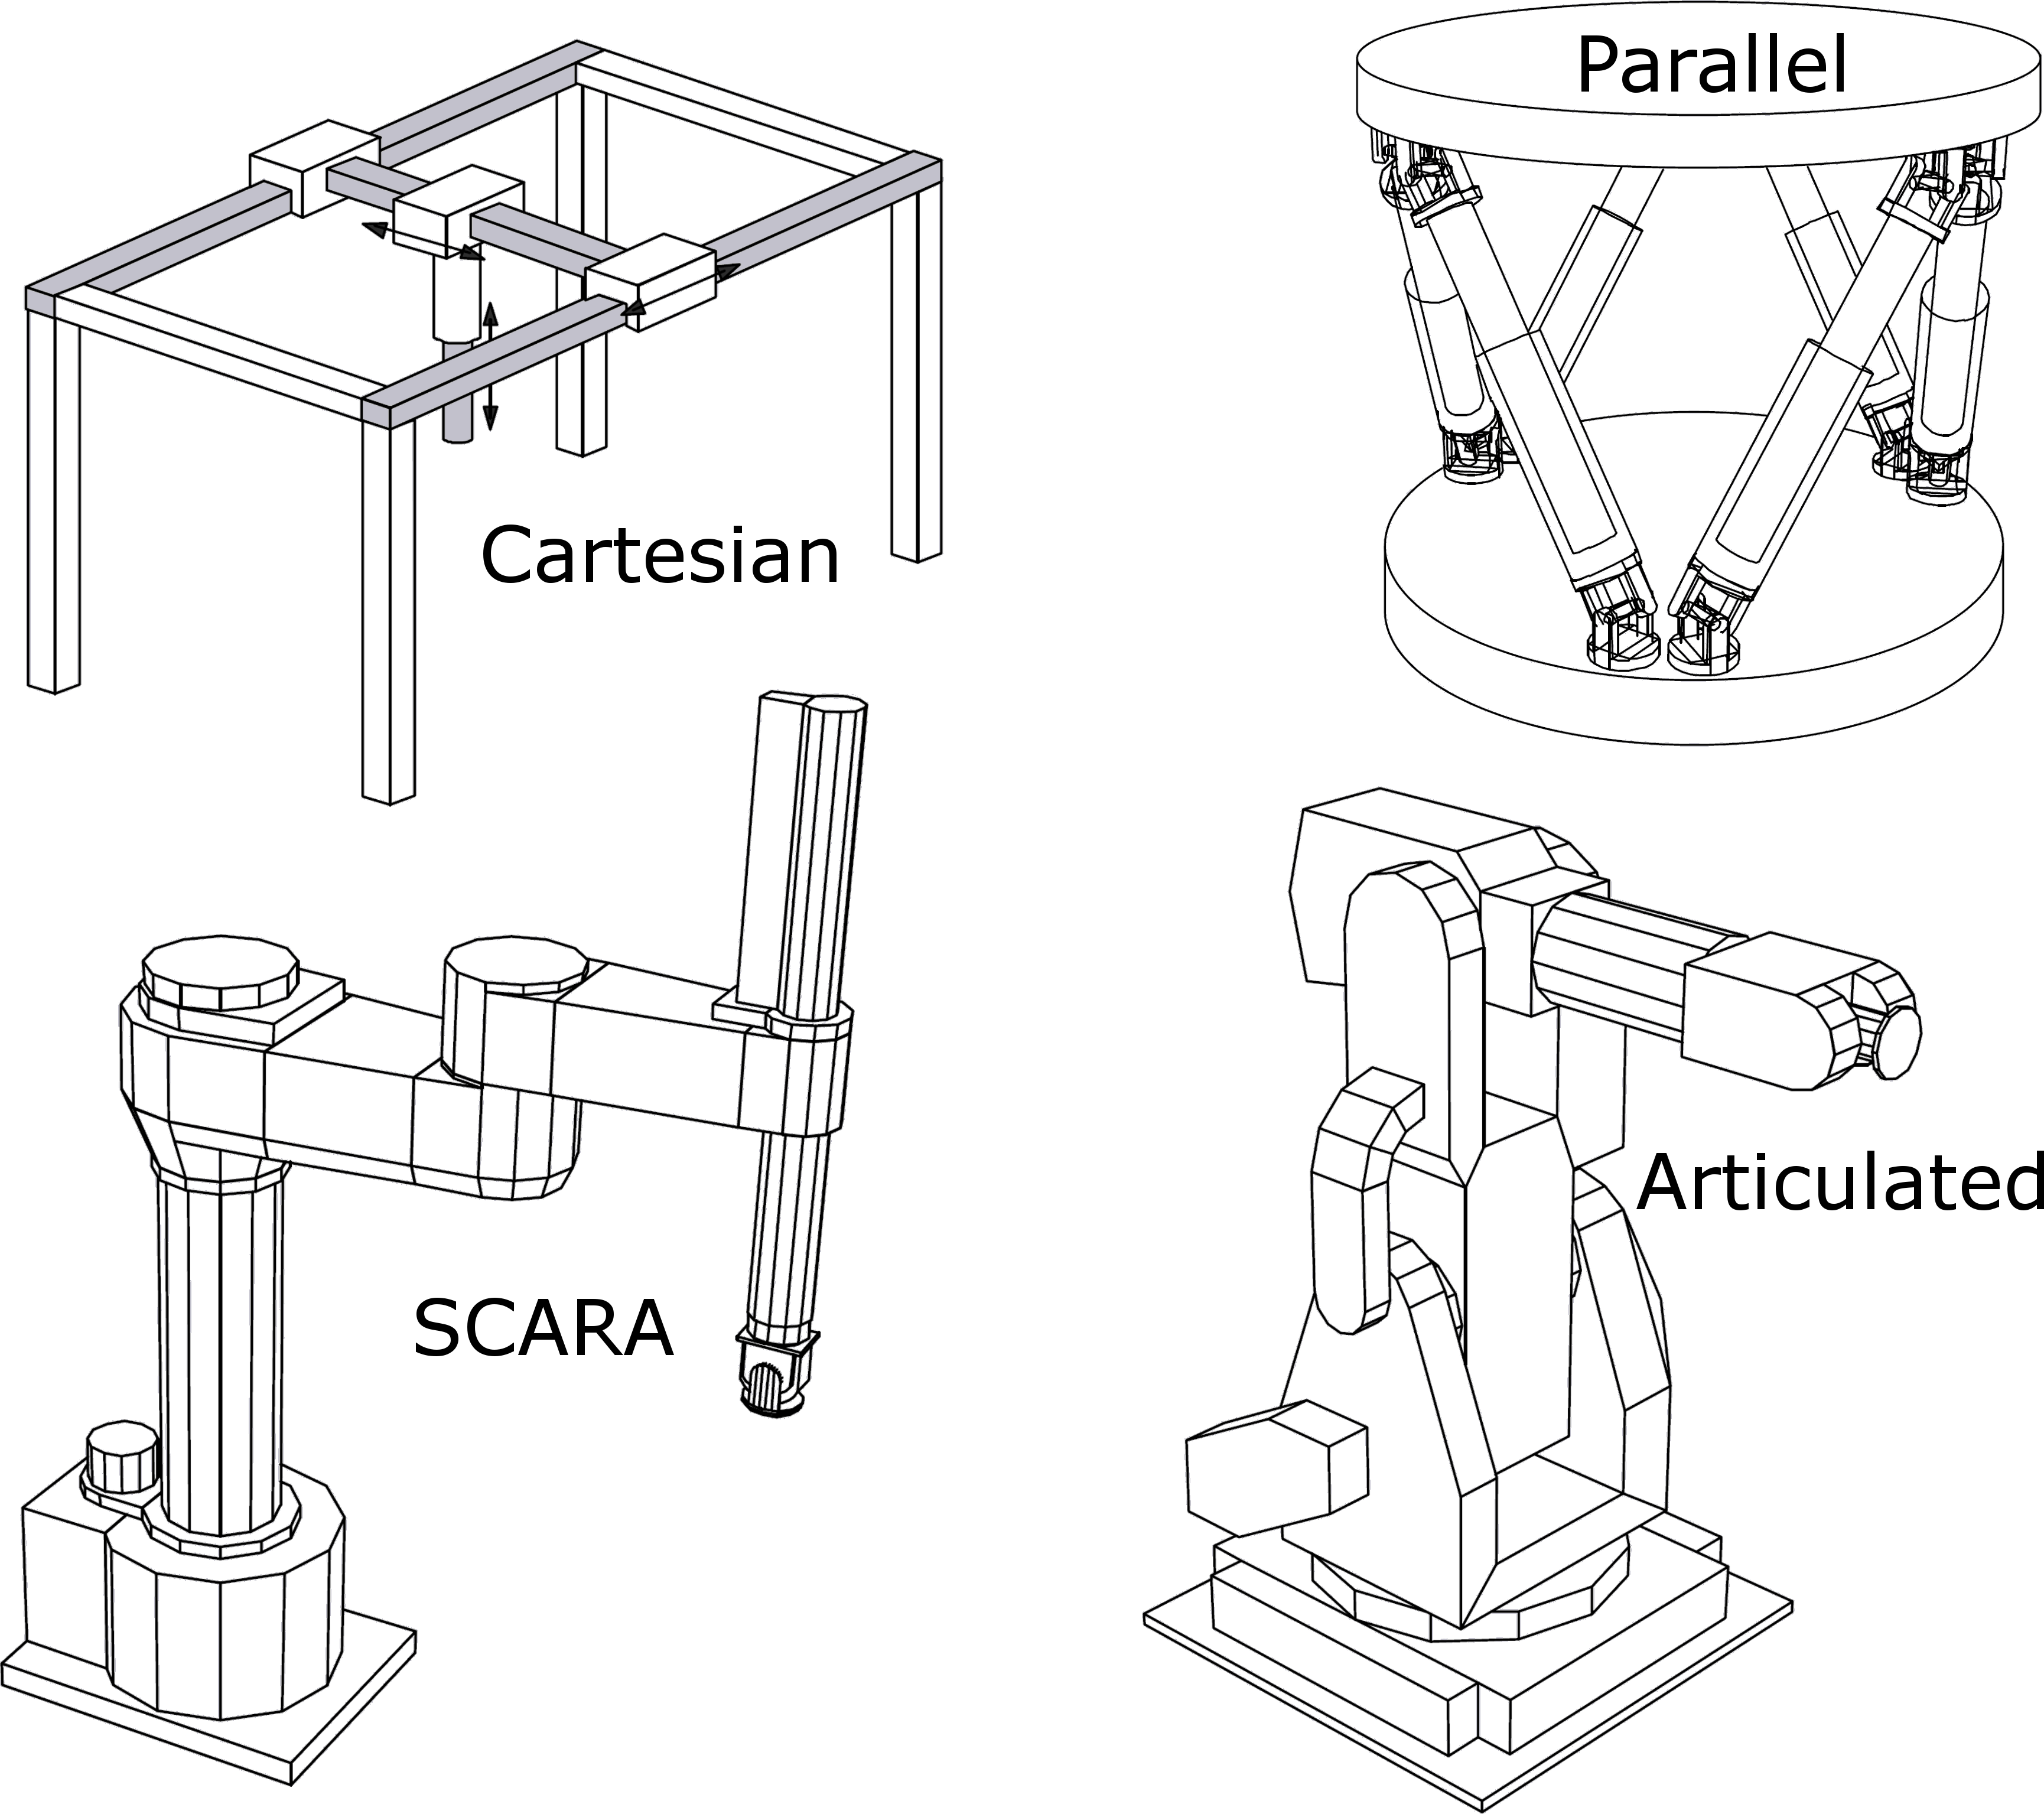
\includegraphics[width=0.785\textwidth]{graphics/andrej/indu_mani}

\tiny{(Springer Handbook of Robotics)}

\end{frame}

\subsection{Safety}
\begin{frame}{Safety}{Risk Assessment and Risk Reduction}
\begin{columns}
\begin{column}{0.05\textwidth}
\end{column}
\begin{column}{0.40\textwidth}
\textbf{Risk Assessment}
    \begin{itemize}
        \item Hazard Identification
        \item Risk Estimation
        \item Risk Evaluation     
    \end{itemize}
\end{column}
\begin{column}{0.25\textwidth}
\begin{figure}[]
    \centering
    
\includegraphics[width=.9\textwidth]{graphics/andrej/arrow}
    \newline
\end{figure}
\end{column}
\begin{column}{0.3\textwidth}
\textbf{Risk Reduction}
\end{column}
\end{columns}
\vspace{10mm}
\centering
\textit{International Organization for Standardization}
\end{frame}

% \begin{frame}{Safety}{\textit{International Organization for Standardization}}
%     \centering
%     \resizebox{\textwidth}{!}{
%     {\begin{tabular}{ll}
%       \hline \rowcolor{beamer@headercolor}\multicolumn{1}{c}{\color{white}{Standard}} & \multicolumn{1}{c}{\color{white}{Scope}} \\ \hline
% \textit{ISO 10218-1:2011} & Robots\\
% \rowcolor{beamer@barcolor} \textit{ISO 10218-2:2011} & Robot systems and integration\\
% \textit{ISO 11161:2007} & Integrated manufacturing systems\\
% \rowcolor{beamer@barcolor} \textit{ISO 11553-1:2005} & Laser processing machines\\
% \textit{ISO 12100:2010} & Risk assessment and risk reduction\\
% \rowcolor{beamer@barcolor} \textit{ISO 13849-1:2015} & Safety-related parts of control systems\\
% \textit{ISO 13850:2015} & Emergency stop function\\
% \rowcolor{beamer@barcolor} \textit{ISO 13854:1996} & Minimum gaps\\
% \textit{ISO 13857:2008} & Safety distances\\
% \rowcolor{beamer@barcolor} \textit{ISO 14119:2013} & Interlocking devices associated with guards\\
% \textit{ISO 14120:2015} & Guards\\
% \rowcolor{beamer@barcolor} \textit{ISO 60825-4:2007} & Laser guards\\
% \hline
%     \end{tabular}}}
% \end{frame}

\section{Final Problem Statement}
\begin{frame}{Final Problem Statement}
\begin{center}
\textbf{
How can a six-axis industrial manipulator and a fibre laser be used to weld the impeller from \textit{Grundfos}' \textit{CR10} pump?
}\end{center}
\end{frame}
\phantomsection
\section{Requirement Specifications}
\begin{frame}{Requirement Specifications}{\textit{Grundfos} Case}
\begin{itemize}
    \item Welding must be performed with an industrial manipulator
    \item Impeller must be stationary during a welding sequence
    \item Cycle time must be within $45.0$ $s$
    \item Robot cell must be no larger than $4\cdot10^{3}$ $\times$ $4\cdot10^{3}$ $mm$
\end{itemize}
\vspace{5mm}
\centering{

\includegraphics[width=0.7\textwidth]{graphics/andrej/grundfos_logo}

\tiny{(grundfos.com)}}
\end{frame}

\begin{frame}{Requirement Specifications}{Laser Welding Equipment}
\begin{columns}
\column{0.55\textwidth}
\begin{itemize}
    \item \textit{HIGHYAG BIMO W}
        \begin{itemize}
            \item Fibre laser processing head
            \item $6.00\cdot10^{3}$ $W$
            \item $4.40$ $kg$
            \item $479 \times 90.0 \times 388$ $mm$
            % \item Onboard camera
        \end{itemize}   
\end{itemize}
\column{0.45\textwidth}
\centering
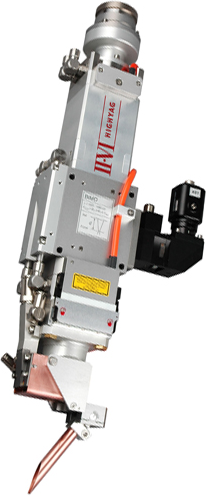
\includegraphics[width=.65\textwidth]{graphics/andrej/bimo}

\tiny{(highyag.com)}
\end{columns}
\end{frame}

%Hello there, I am sorry for the intrusion and interruption, kind sir, but I was hoping you could help me out with a slight problem I am experiencing. You see, I wish to insert a table, where each row is of interchanging colors, I am able to do so, even with the colors that I wish to use, however, due to my lack of experience in the area, I cannot do it in a proper manor. So far, I am inserting "\definecolor{colorK}{HTML}{DEDEDE}" just before I use it, with no problems. I do however wish to insert it, so that it affects the entire file. I believe the proper way is to insert it somewhere like in the "aausidebartheme" and in the preamble insert "\userpackage{color}", but I would require assistance in this. 

\begin{frame}{Requirement Specifications}{Design and Performance Requirements}
    \centering
    \resizebox{\textwidth}{!}{
    \begin{tabular}{l}
    \hline
    \rowcolor{beamer@headercolor} \multicolumn{1}{c}{\color{white}{Design Requirements}} \\
    \hline
    Dimension of the workspace must be at most $4\cdot10^{3}$ $\times$ $4\cdot10^{3}$ $mm$ \\
    \rowcolor{beamer@barcolor} Workcell safety must meet \textit{ISO} standards\\   
    Workcell must be equipped with a suitable industrial manipulator\\
    \rowcolor{beamer@barcolor} Material flow must happen without human aid\\
    Sub-components must be held in a fixed position\\
    \hline
    \end{tabular}}

\vspace{5mm}

    \resizebox{\textwidth}{!}{
    \begin{tabular}{l}
    \hline
    \rowcolor{beamer@headercolor} \multicolumn{1}{c}{\color{white}{Performance Requirements}} \\
    \hline
    Cycle time must be no more than $45.0$ $s$\\
    \rowcolor{beamer@barcolor} Welding velocity must be kept constant at $167$ $mm/s$.\\
    Relative distance must be constant at $480$ $mm$\\
    \rowcolor{beamer@barcolor} The industrial manipulator must have at least five degrees of freedom.\\
    Relative angle must be perpendicular during vane welding.\\
    \rowcolor{beamer@barcolor} Relative angle during hub welding must be $30.0\degree$\\ %enable math symbols
    Deviation must not exceed $0.300$ $mm$\\
    \hline
    \end{tabular}}
    \centering
\end{frame}
\phantomsection
\section{Design}
\begin{frame}{Design of the \textit{CORPS}}
\begin{columns}
\column{0.4\textwidth}
    \begin{itemize}
        \item \textit{HIGHYAG BIMO W}
        \item Industrial manipulator
        \item Conveyor
        \item Fixture
        \item Safety measures
    \end{itemize}
\column{0.6\textwidth}
\centering{
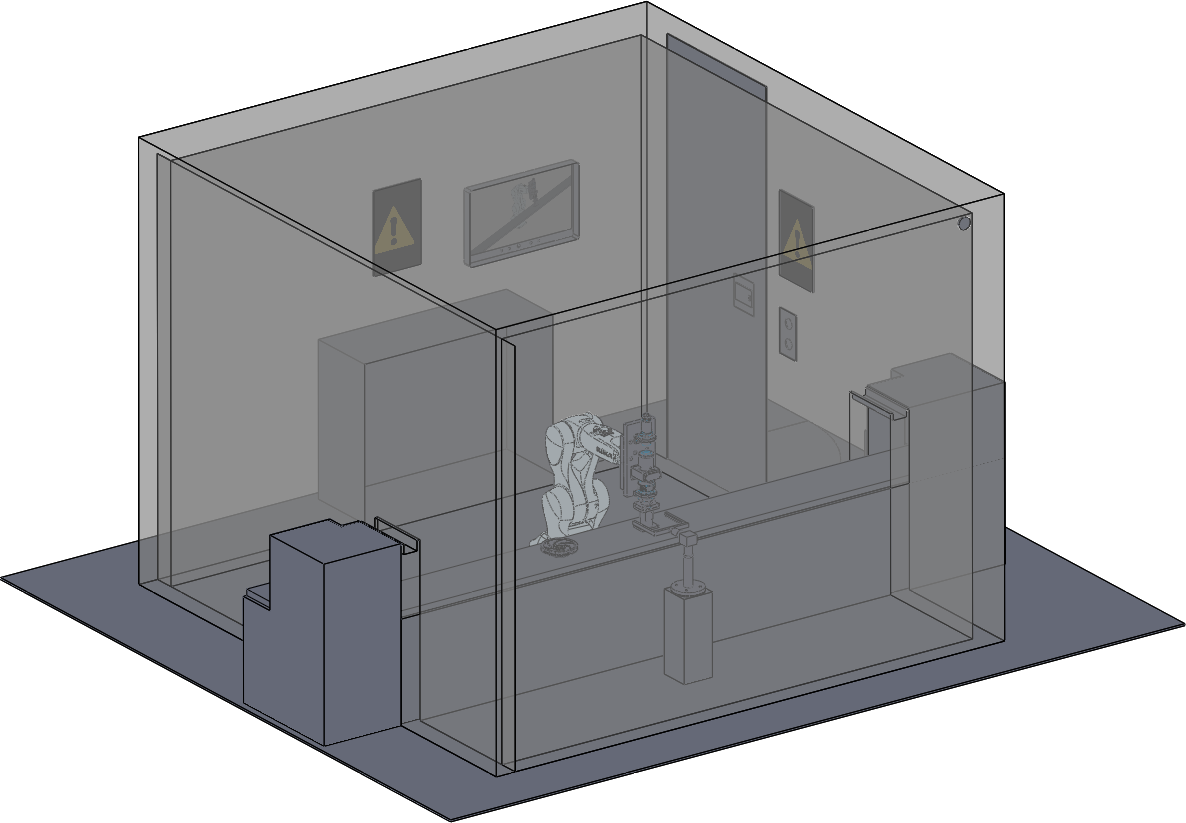
\includegraphics[width=\textwidth]{graphics/andrej/workcell_front_side}}
\end{columns}
\end{frame}




% \begin{frame}{Selection of Industrial Manipulator}{Market Investigation}
% \centering{
% \includegraphics[width=.975\textwidth]{graphics/andrej/market_analysis}

% \tiny{(abb.com) (cloosrobot.com)}}
% \end{frame}

\begin{frame}{Selection of Industrial Manipulator}
\begin{columns}
\column{.55\textwidth}
    \begin{itemize}
        \item Market investigation
    \vspace{2.5mm}
        \item \textit{Grundfos}
            \begin{itemize}
                \item Ease the implementation
                \item Reduce the costs
            \end{itemize}
    \vspace{2.5mm}
        \item \textit{KUKA KR 6 R700 sixx}
            \begin{itemize}
                \item Maximum payload - $6.00$ $kg$
                \item Reach - $707$ $mm$
                \item Repeatability - $30.0\cdot10^{-3}$ $mm$
            \end{itemize}
    \end{itemize}
\column{.45\textwidth}
\centering{
\includegraphics[width=0.815\textwidth]{graphics/andrej/kuka}

\tiny{(kuka.com)}}
\end{columns}
\end{frame}

\begin{frame}{Selection of Conveyor System}
    \begin{itemize}
        \item Chain conveyor
            \begin{itemize}
                \item \textit{CALDAN CONVEYOR A/S}
            \end{itemize}
    \end{itemize}
\vspace{5mm}
\centering{
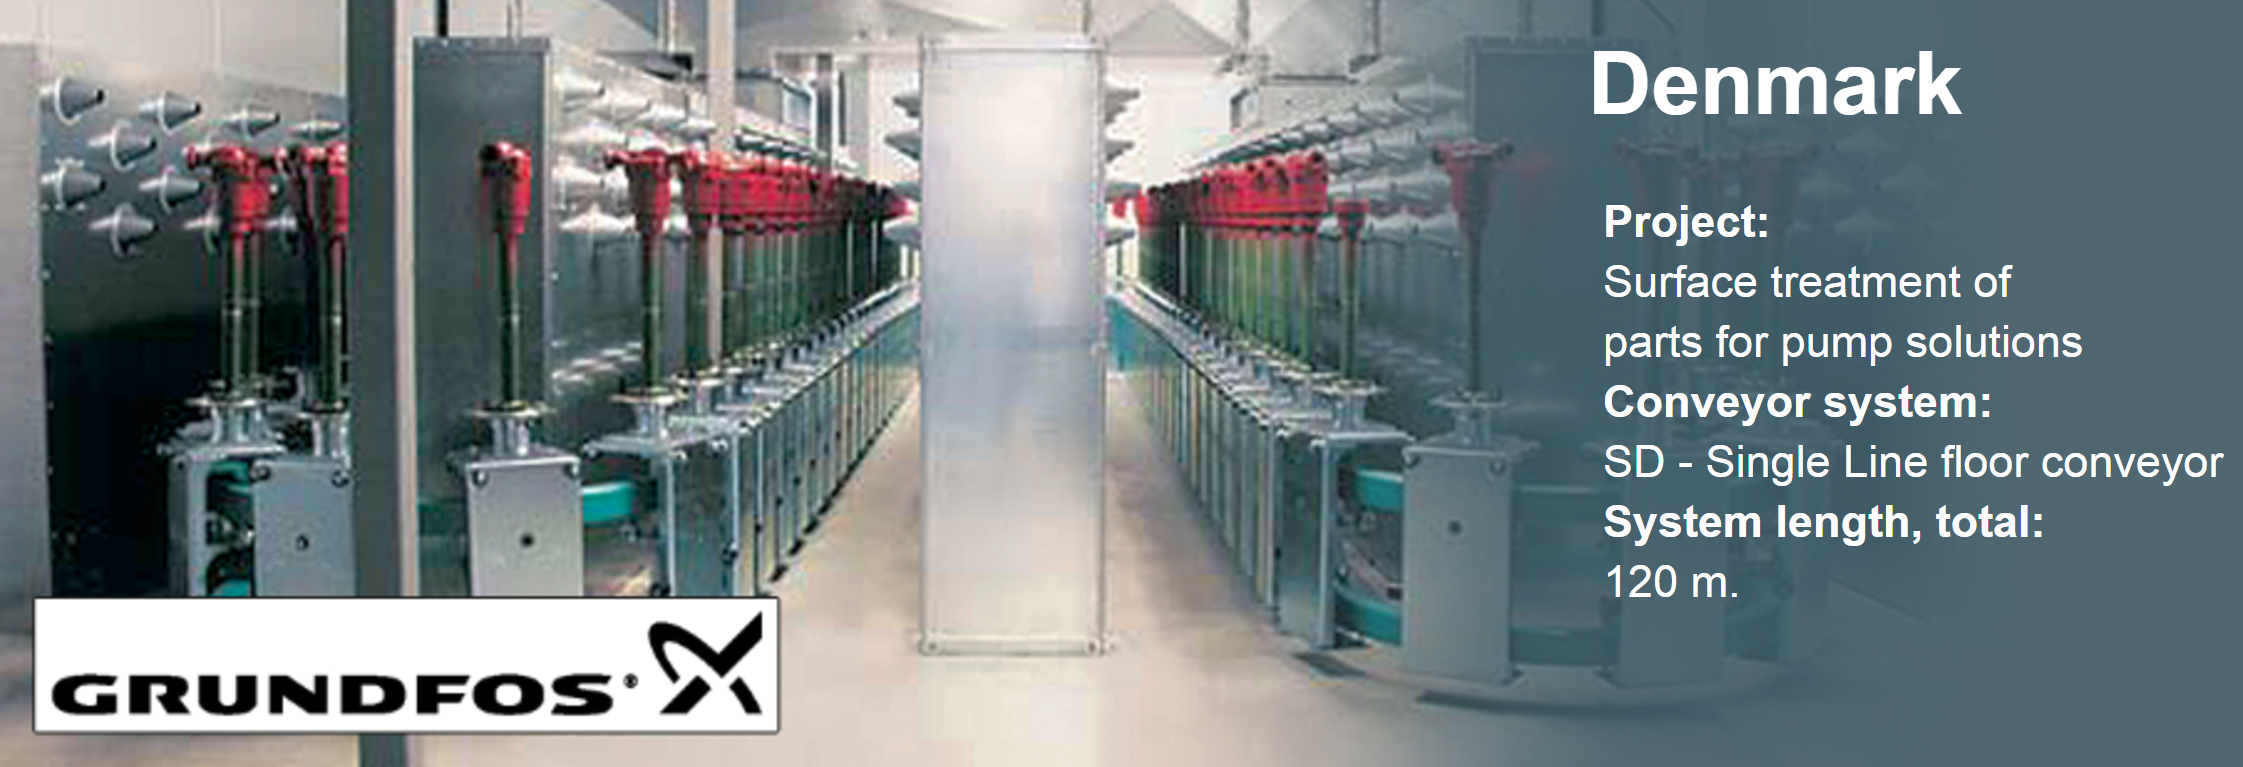
\includegraphics[width=0.9\textwidth]{graphics/andrej/conveyor}

\tiny{(caldan.dk)}}
\end{frame}


\begin{frame}{Fixture}{Design Suggestion}
\begin{itemize}
    \item Accessible welding trajectories
    \item Clamps securing the vanes
    \item Flippable
\end{itemize}

% \begin{columns}
% \column{.5\textwidth}
%   \centering
%   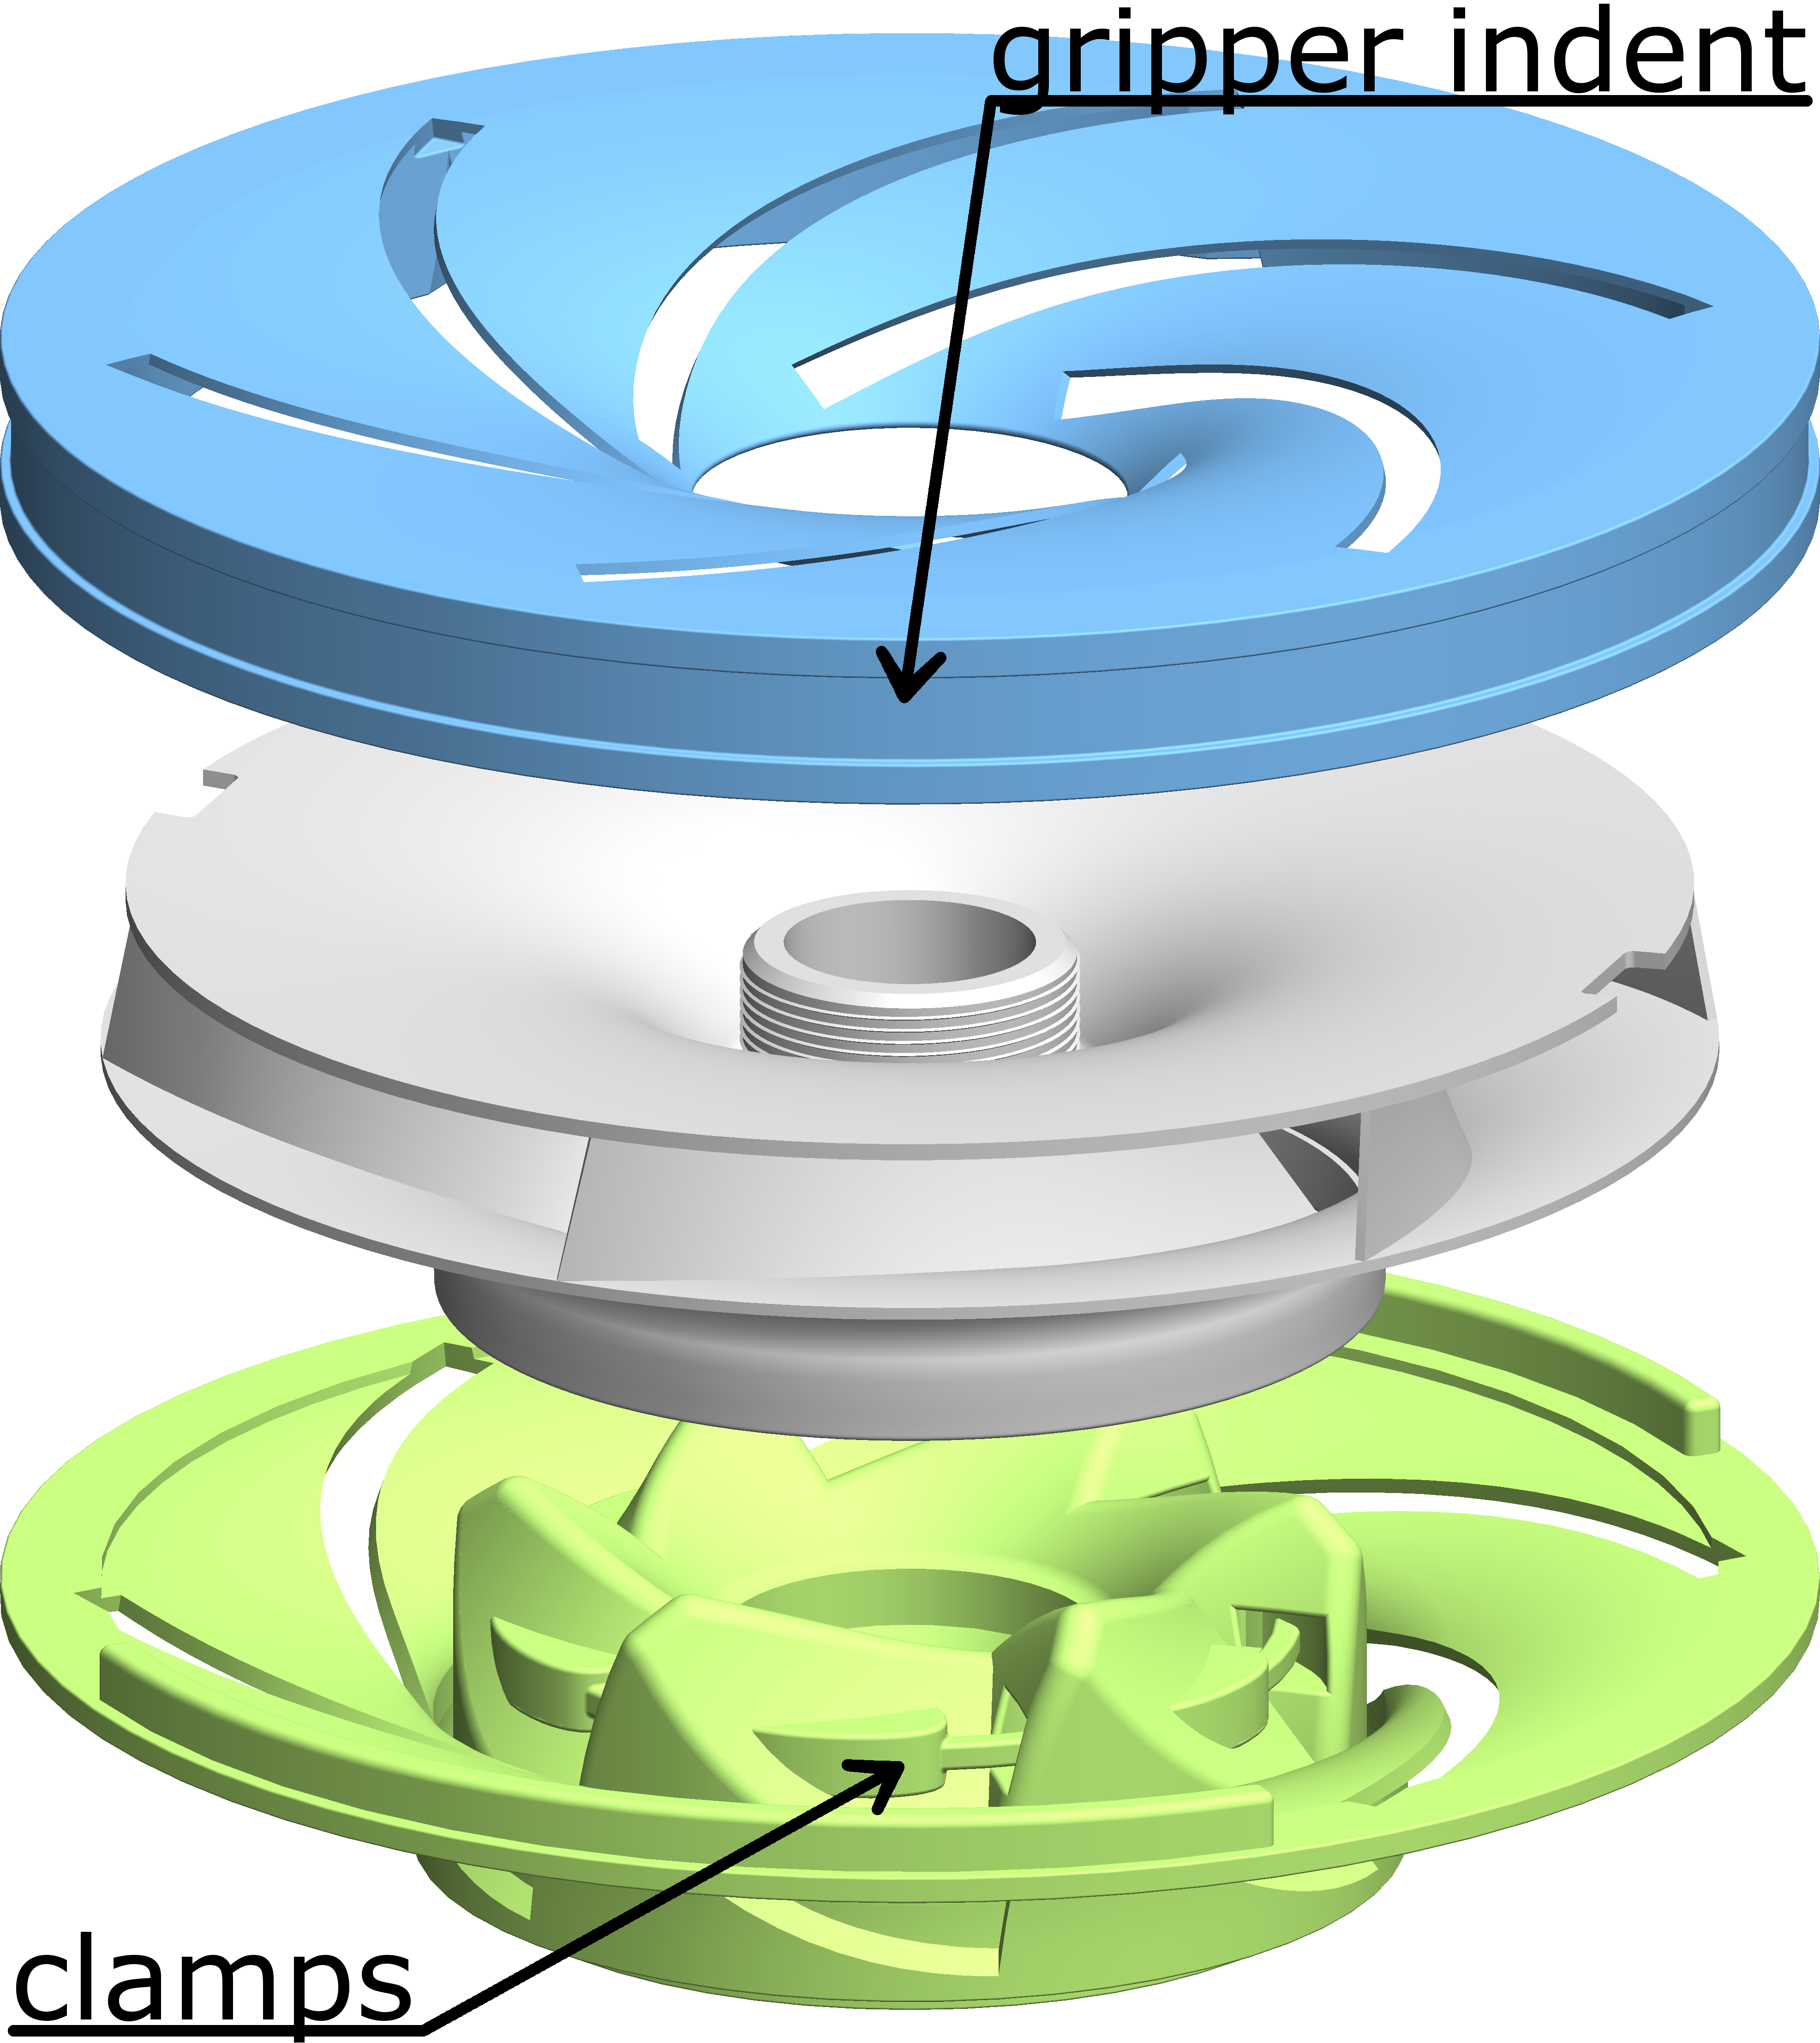
\includegraphics[width=.85\textwidth]{graphics/andrej/if_top}
% \column{.5\textwidth}
%   \centering
%     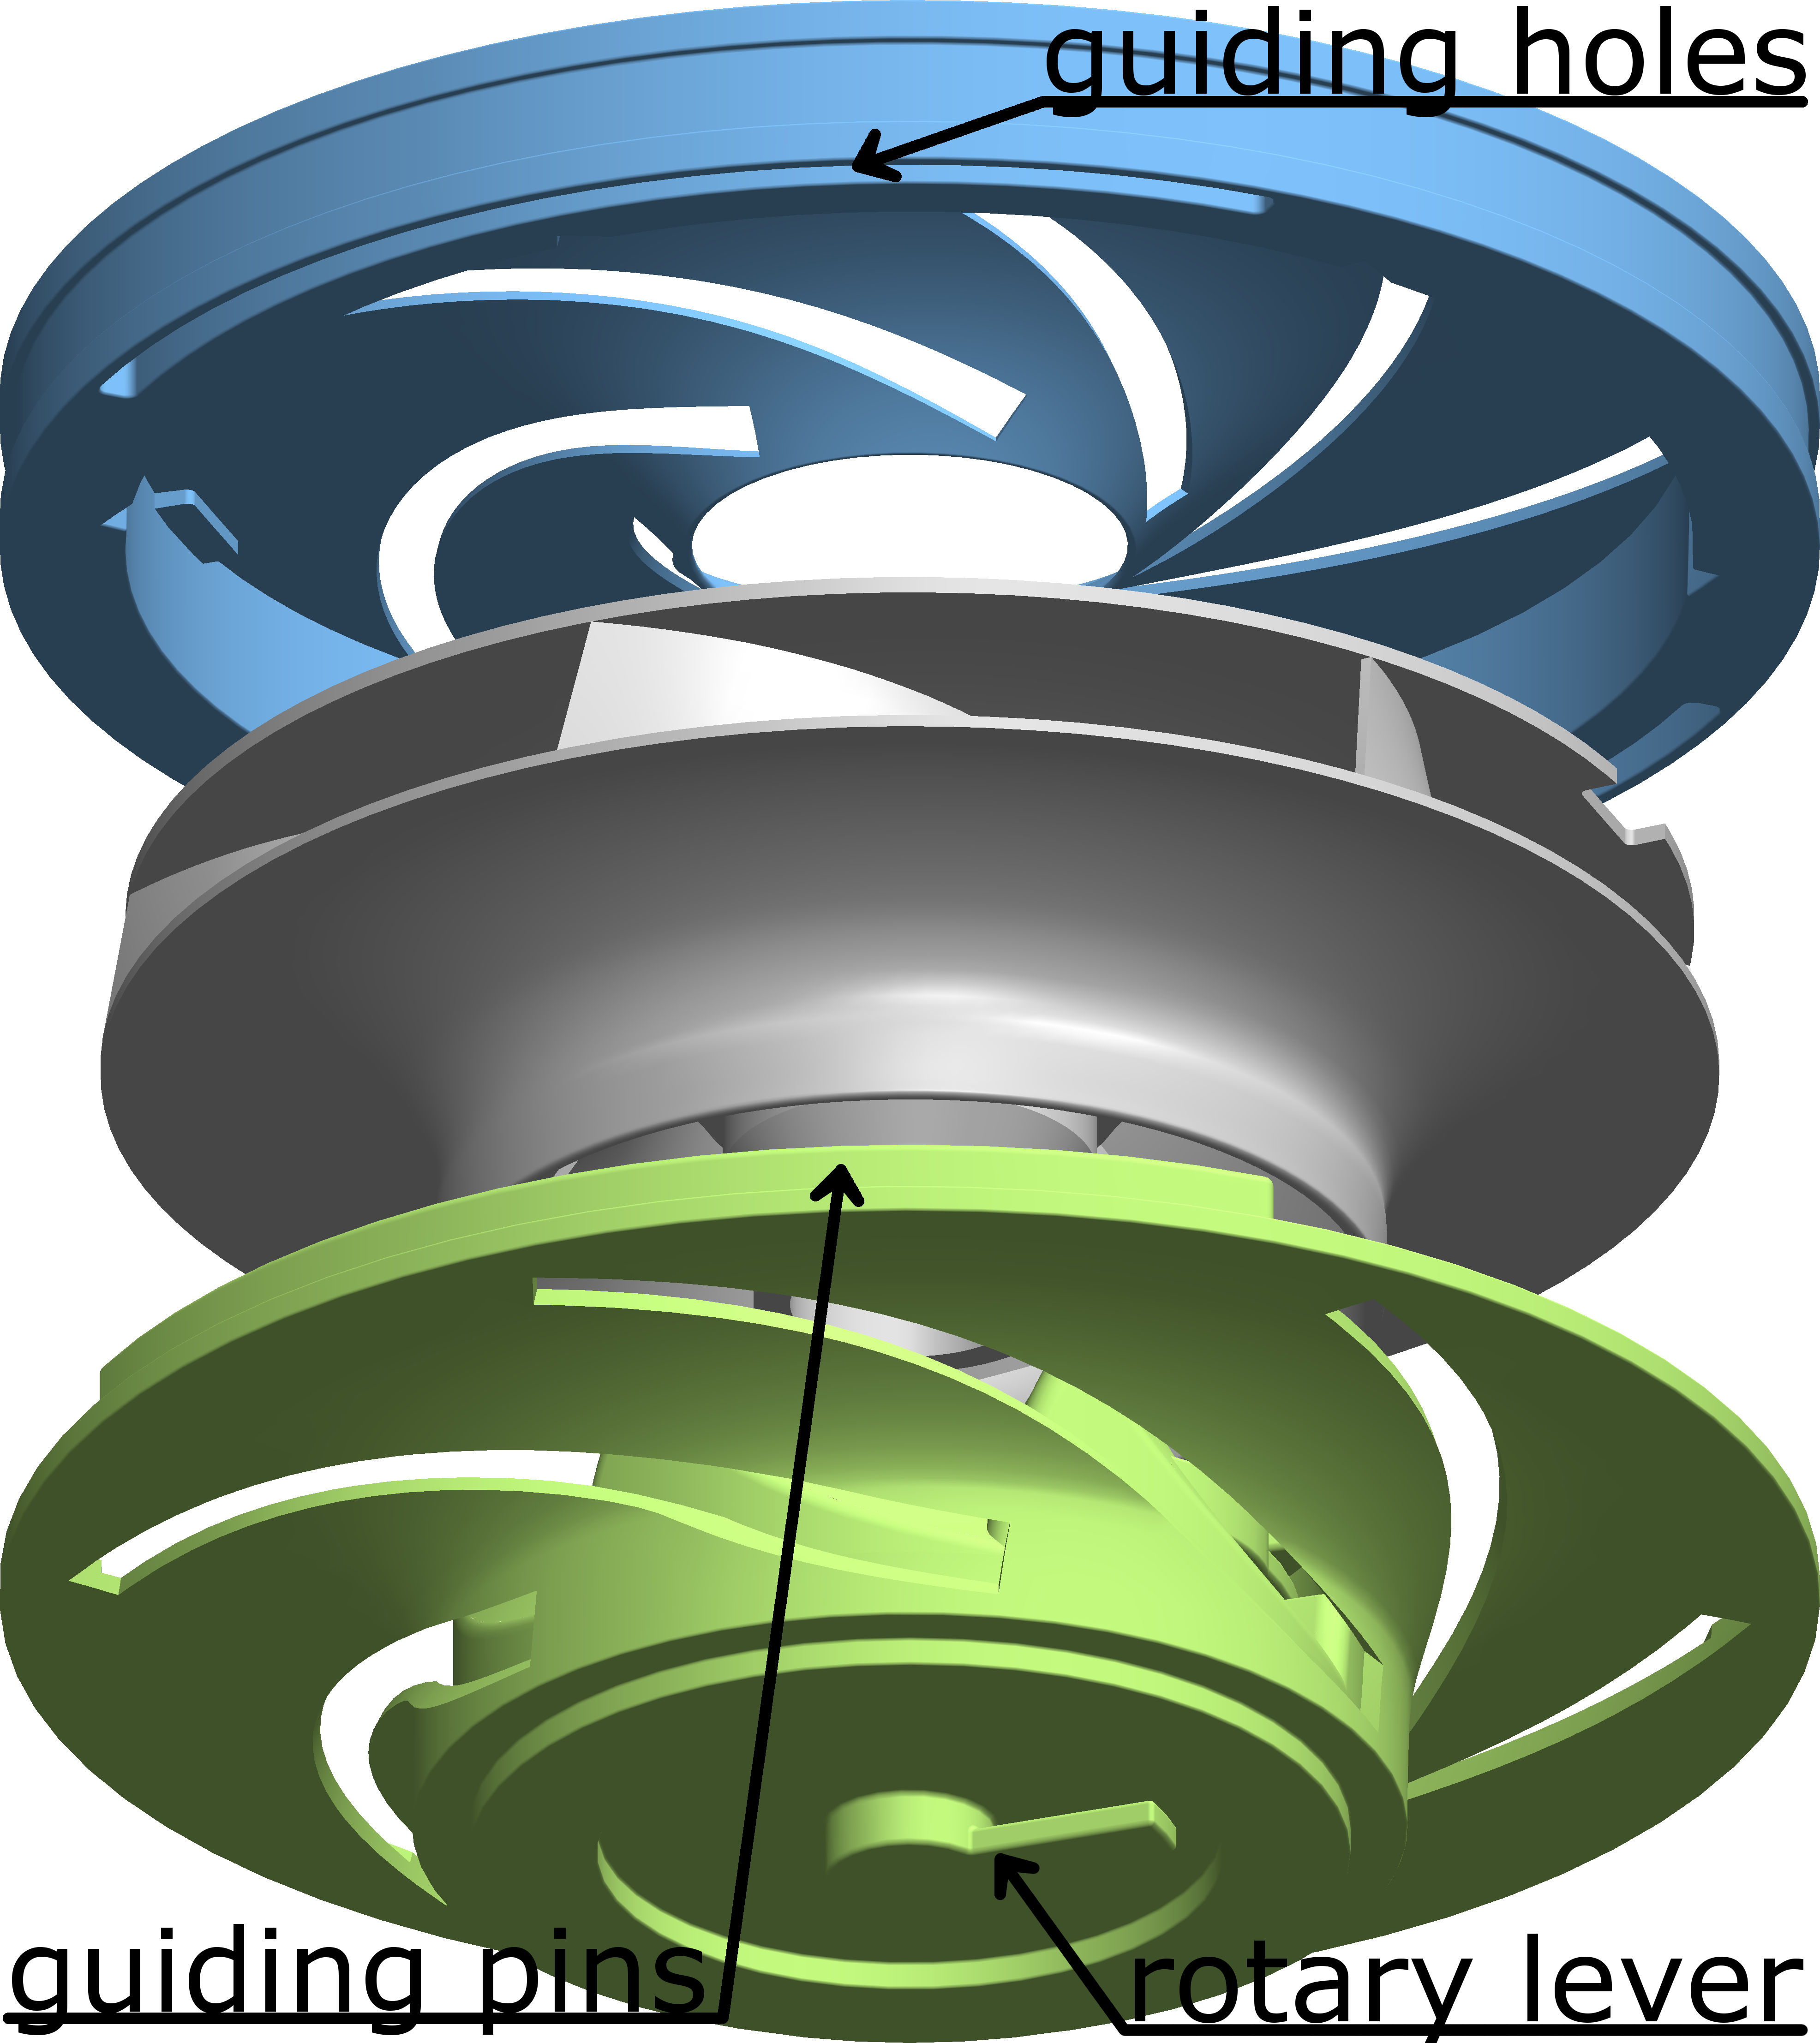
\includegraphics[width=.85\textwidth]{graphics/andrej/if_bottom}
% \end{columns}

\centering{

\includegraphics[width=.9\textwidth]{graphics/andrej/if_cut}}

\end{frame}

\begin{frame}{ATTEMPT2: Fixture}{Design Suggestion}
\begin{itemize}
    \item Accessible welding trajectories
    \item Clamps securing the vanes
    \item Flippable
\end{itemize}

% \begin{columns}
% \column{.5\textwidth}
%   \centering
%   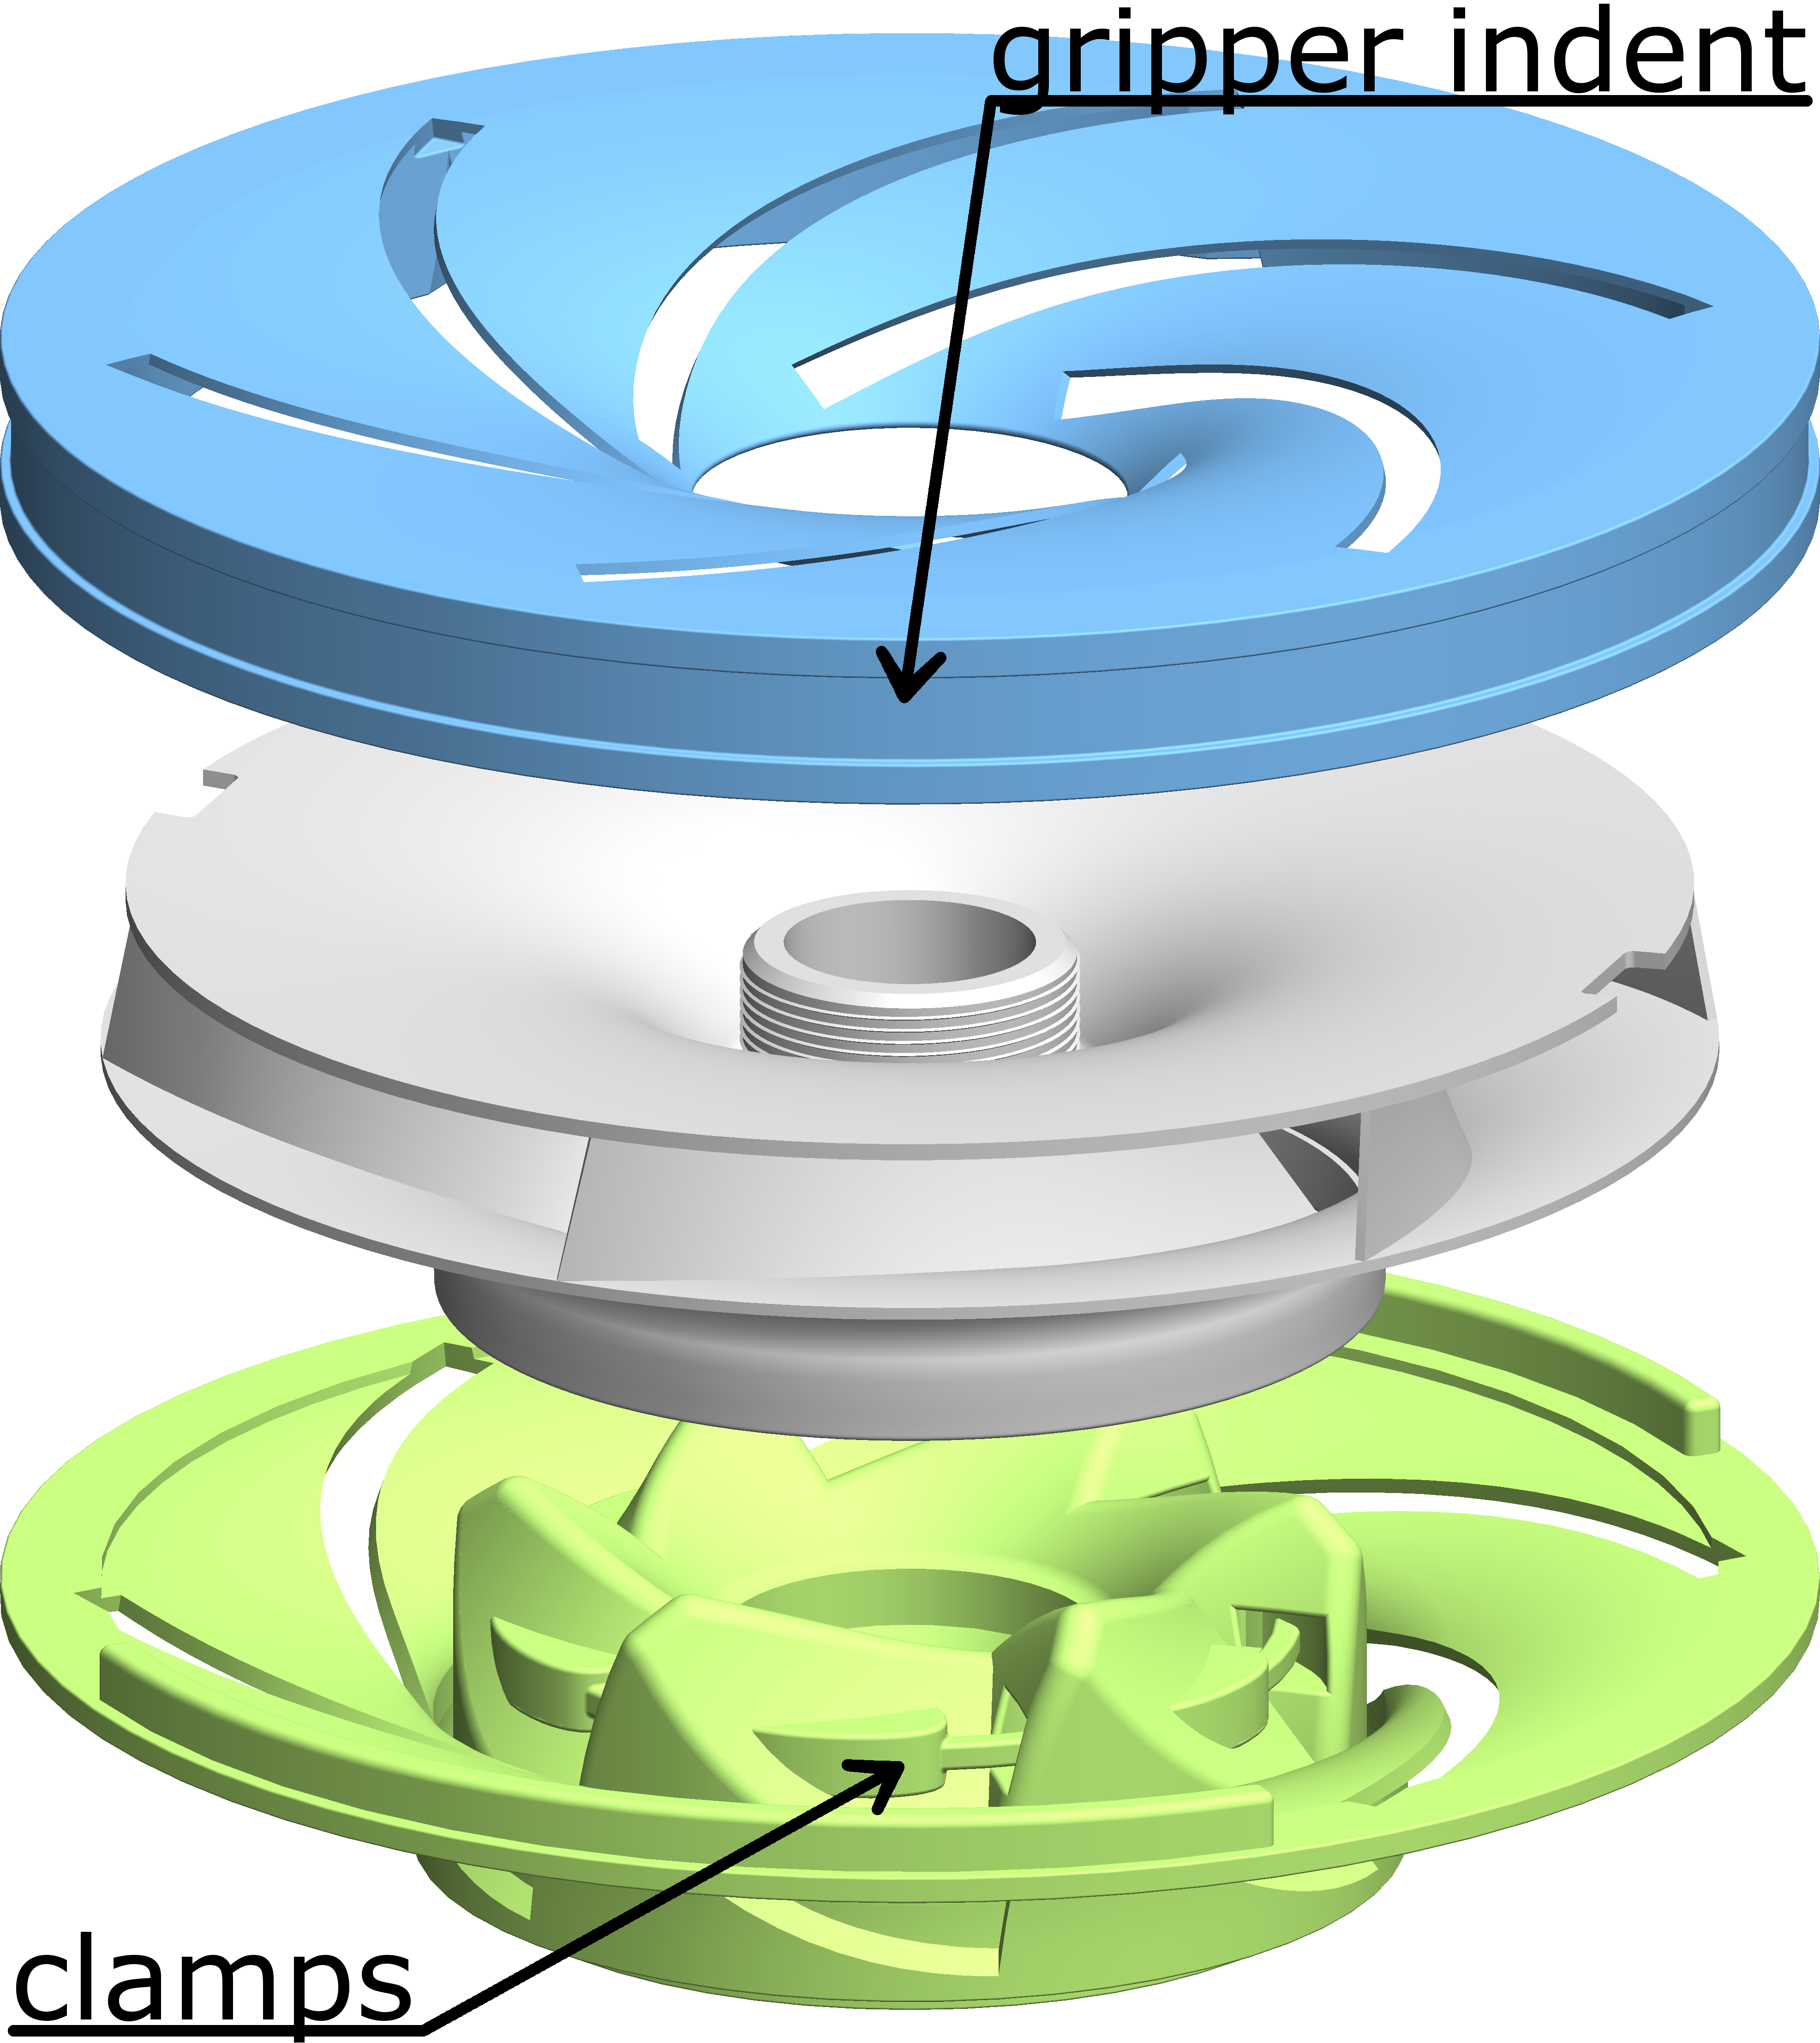
\includegraphics[width=.85\textwidth]{graphics/andrej/if_top}
% \column{.5\textwidth}
%   \centering
%     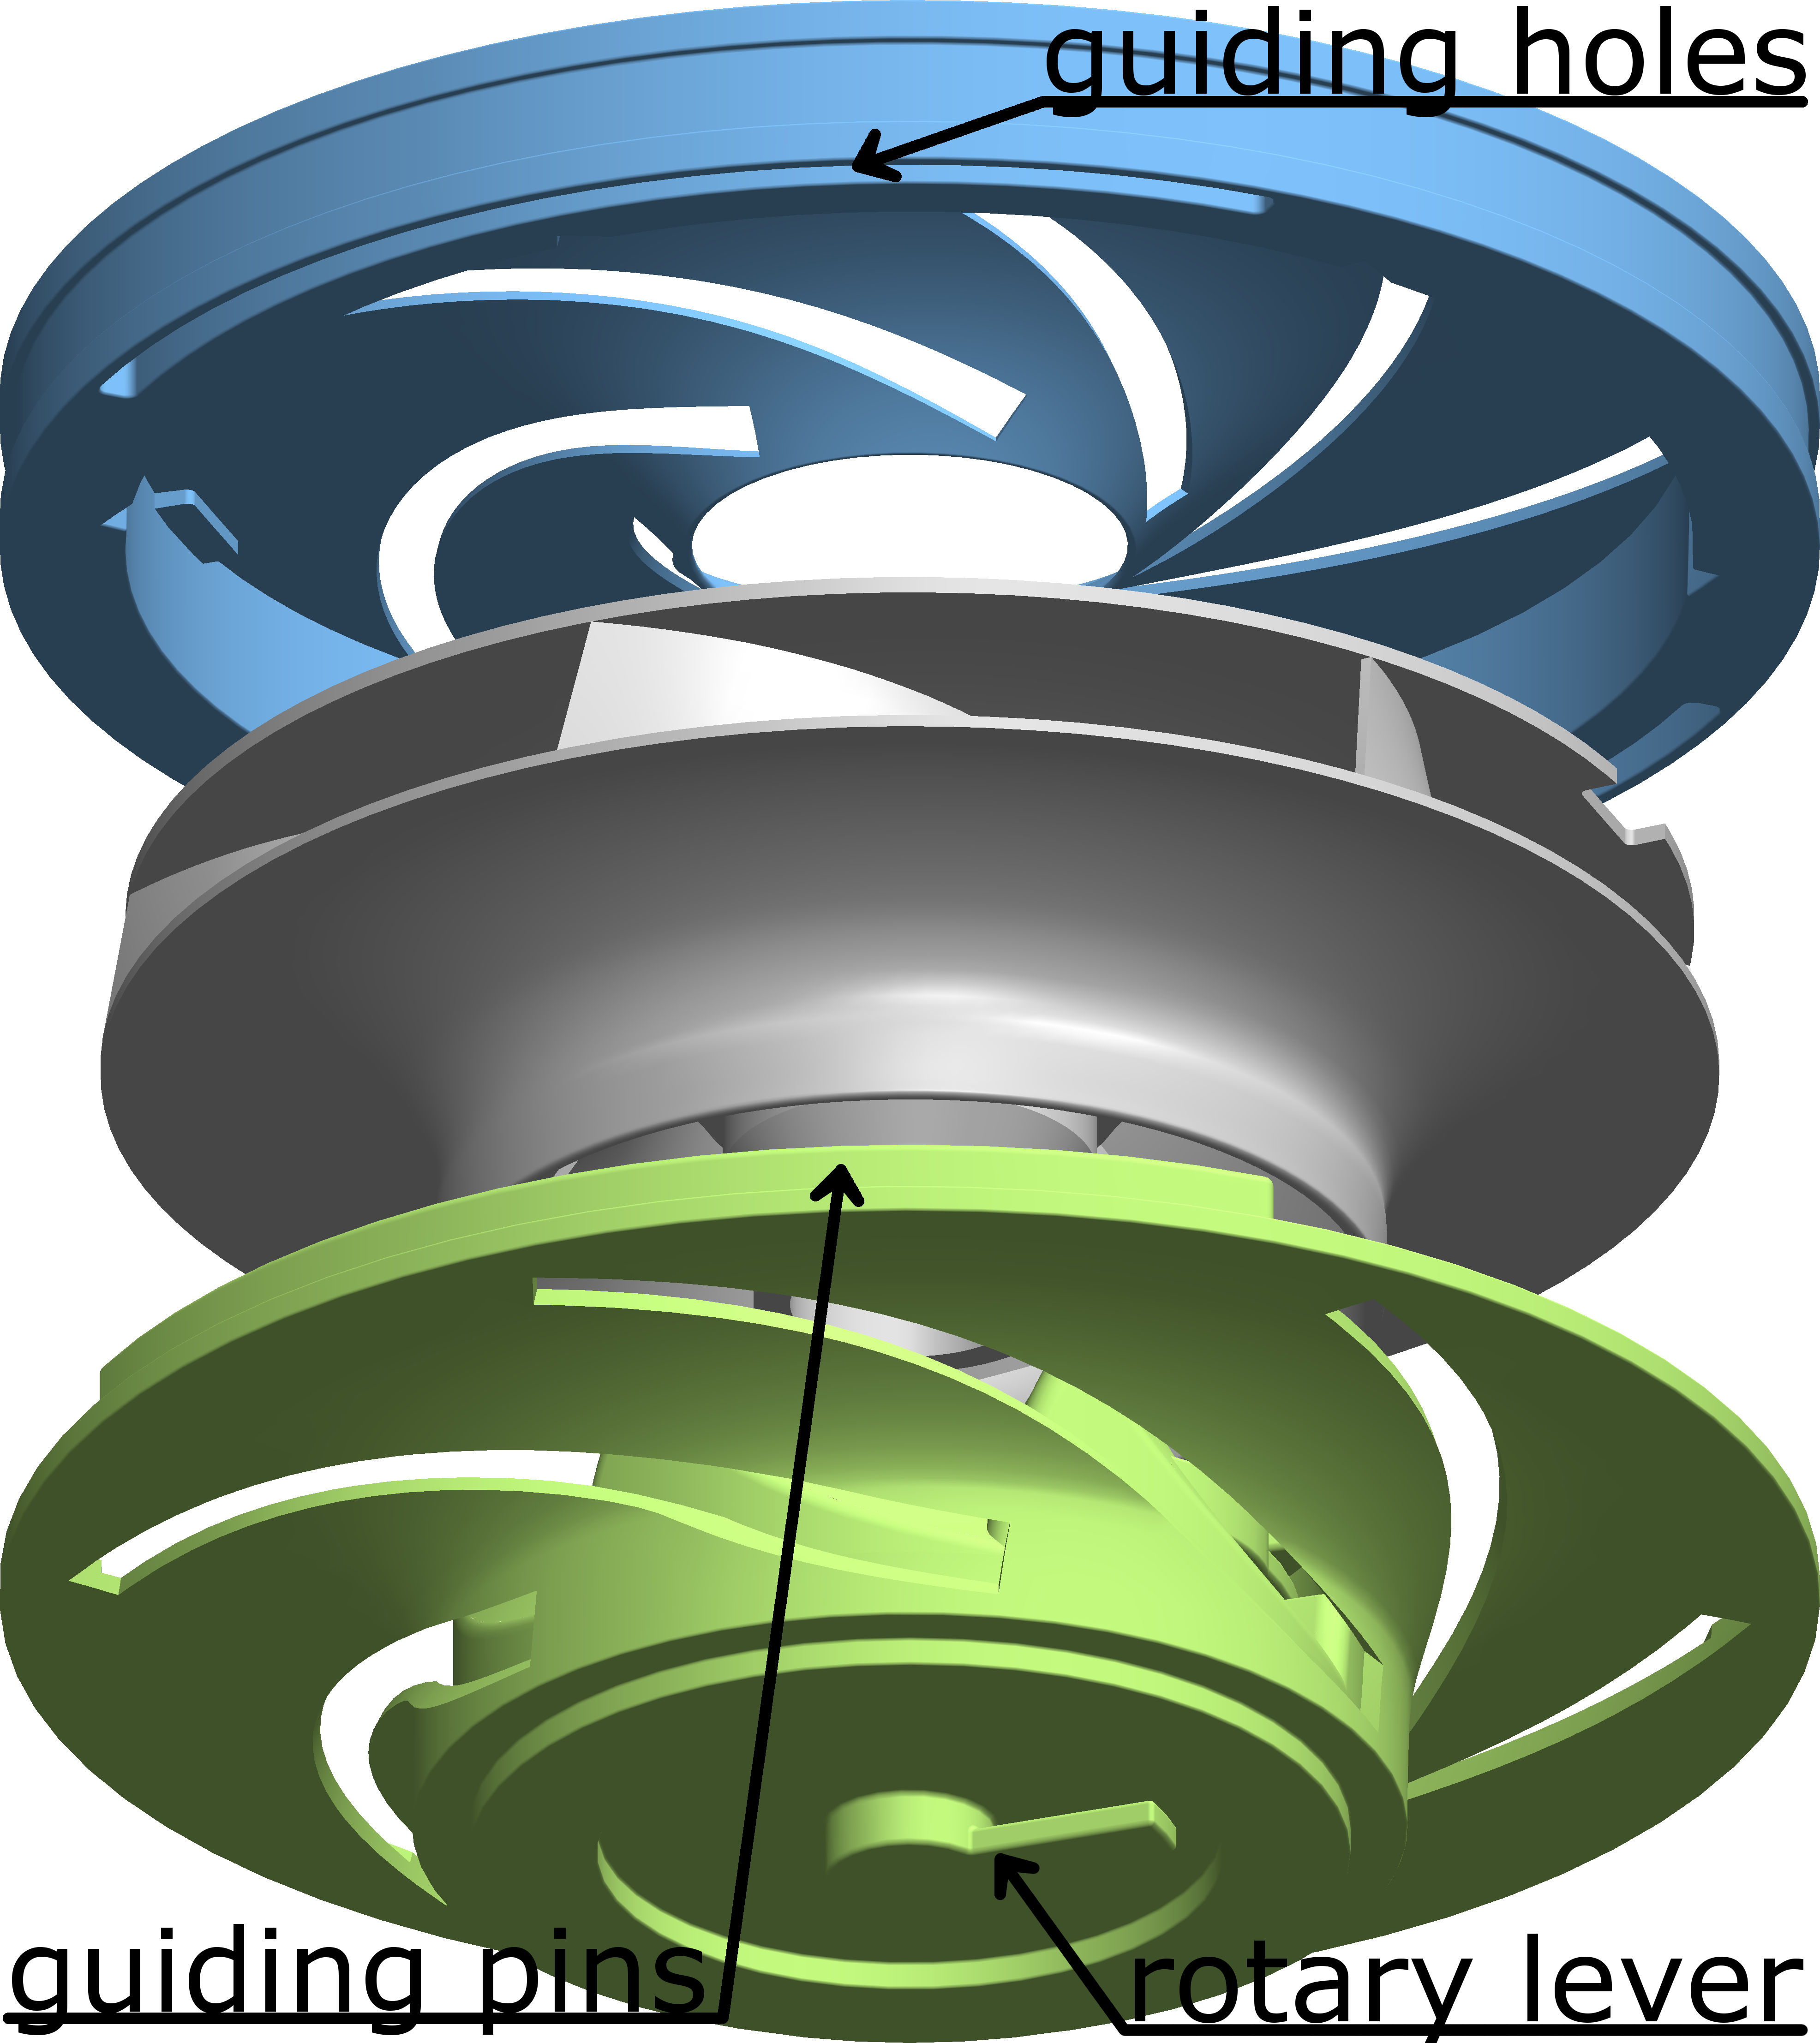
\includegraphics[width=.85\textwidth]{graphics/andrej/if_bottom}
% \end{columns}

\centering{
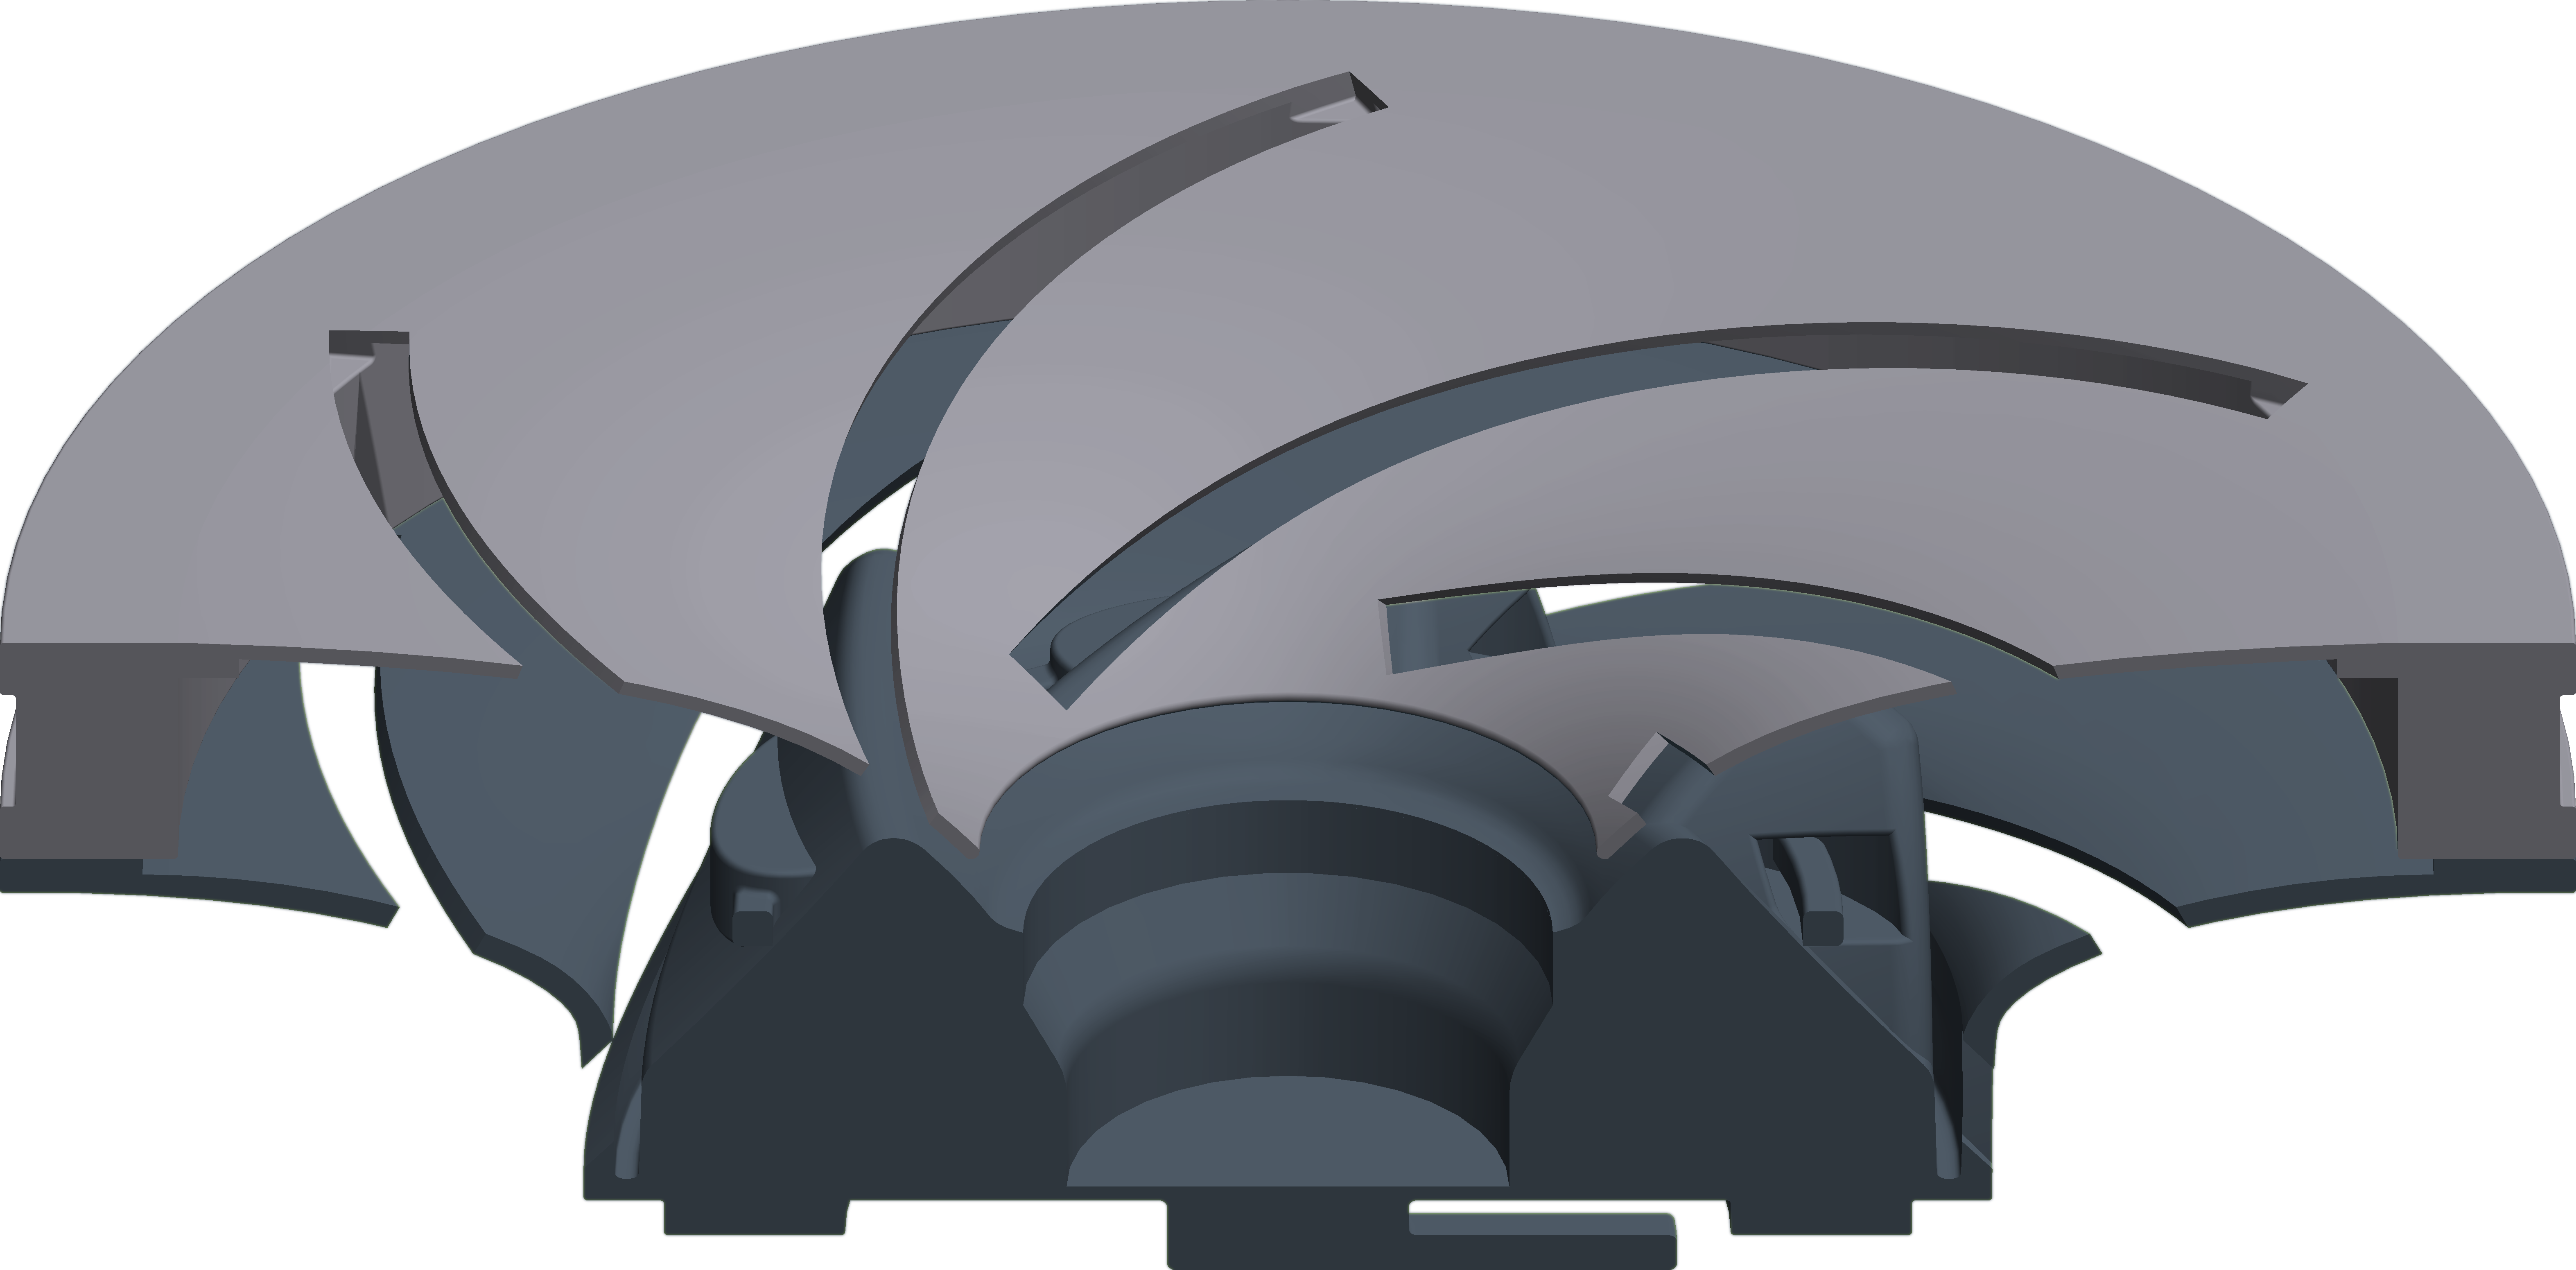
\includegraphics[width=.9\textwidth]{graphics/andrej/if_cut_beamer}}

\end{frame}

\begin{frame}{Fixture}{Fixture Flipping and Fixing System}
 \centering
    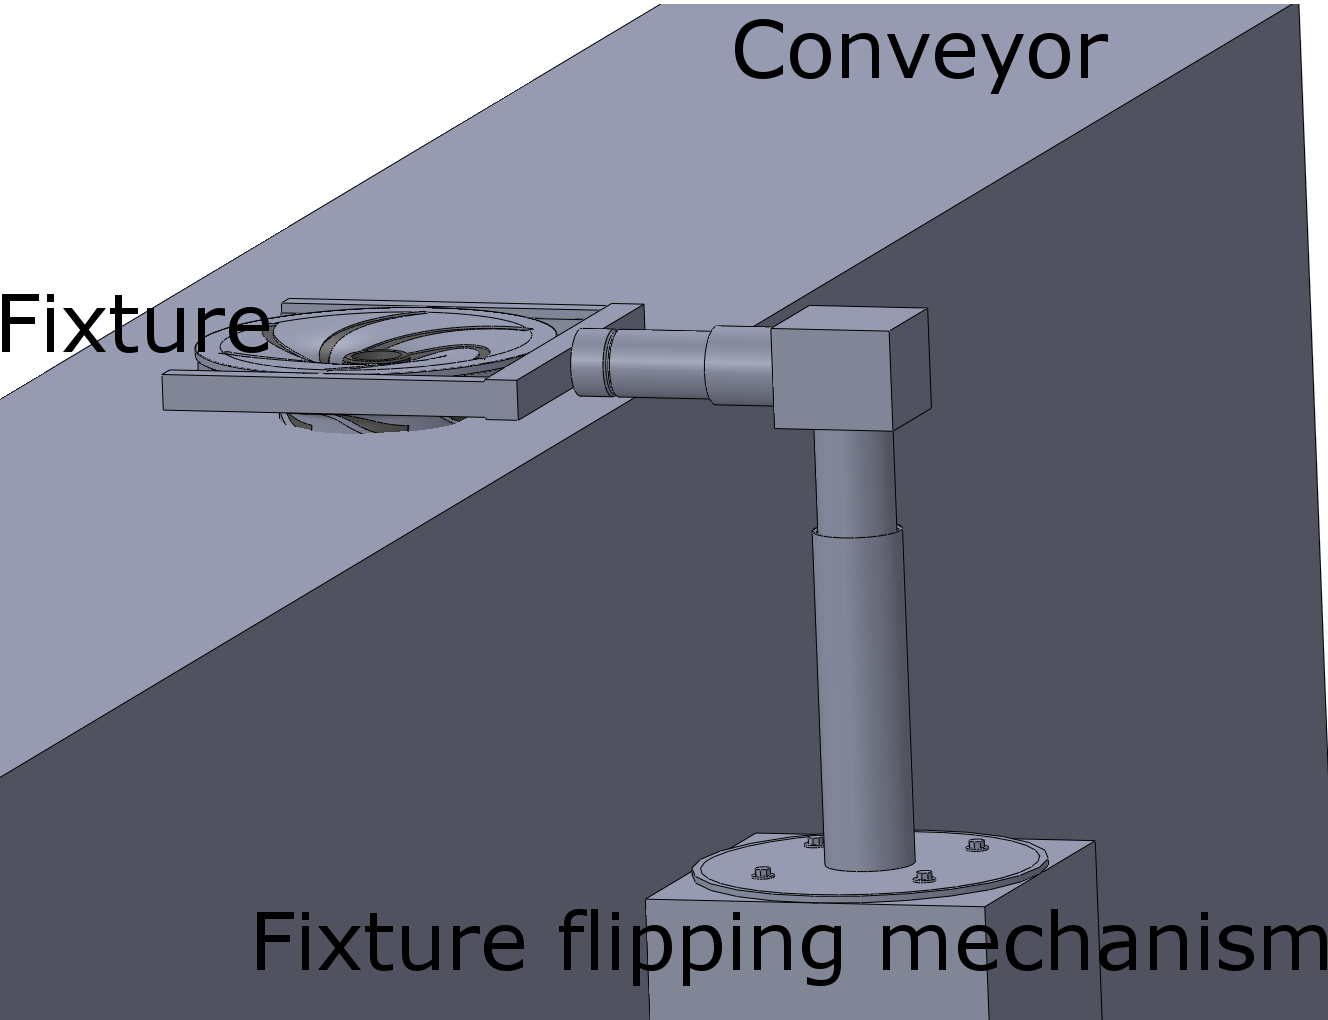
\includegraphics[width=0.9\textwidth]{graphics/andrej/fixture_flipping_mechanism}

\end{frame}














\phantomsection
\section{Mathematics and Programming}
\begin{frame}{Kinematic Model}{Aleksandra Zasadni}
\begin{columns}
\column{0.4\textwidth}
    \begin{itemize}
        \item Mathematical Model 
        \begin{itemize}
            \item Behaviour
            \item Tasks
        \end{itemize}
        \item Kinematic model
    \end{itemize}    
\column{0.6\textwidth}
\centering{
\includegraphics[scale=0.17]{graphics/andrej/kuka}}

\tiny{(kuka.com)}
\end{columns}
\end{frame}

\begin{frame}{Kinematic Model}{Forward Kinematics}
\begin{columns}
\column{0.5\textwidth}
\begin{itemize}
    \item End-effector
    \item Joint variables
    \item Rigid transformation
    \item Separate rigid transform
    \item Denavit-Hartenberg
    \begin{itemize}
        \item Joint matrices
        \item Link matrices
        \item Standardised
    \end{itemize}
\end{itemize}
\column{0.5\textwidth}
\centering{
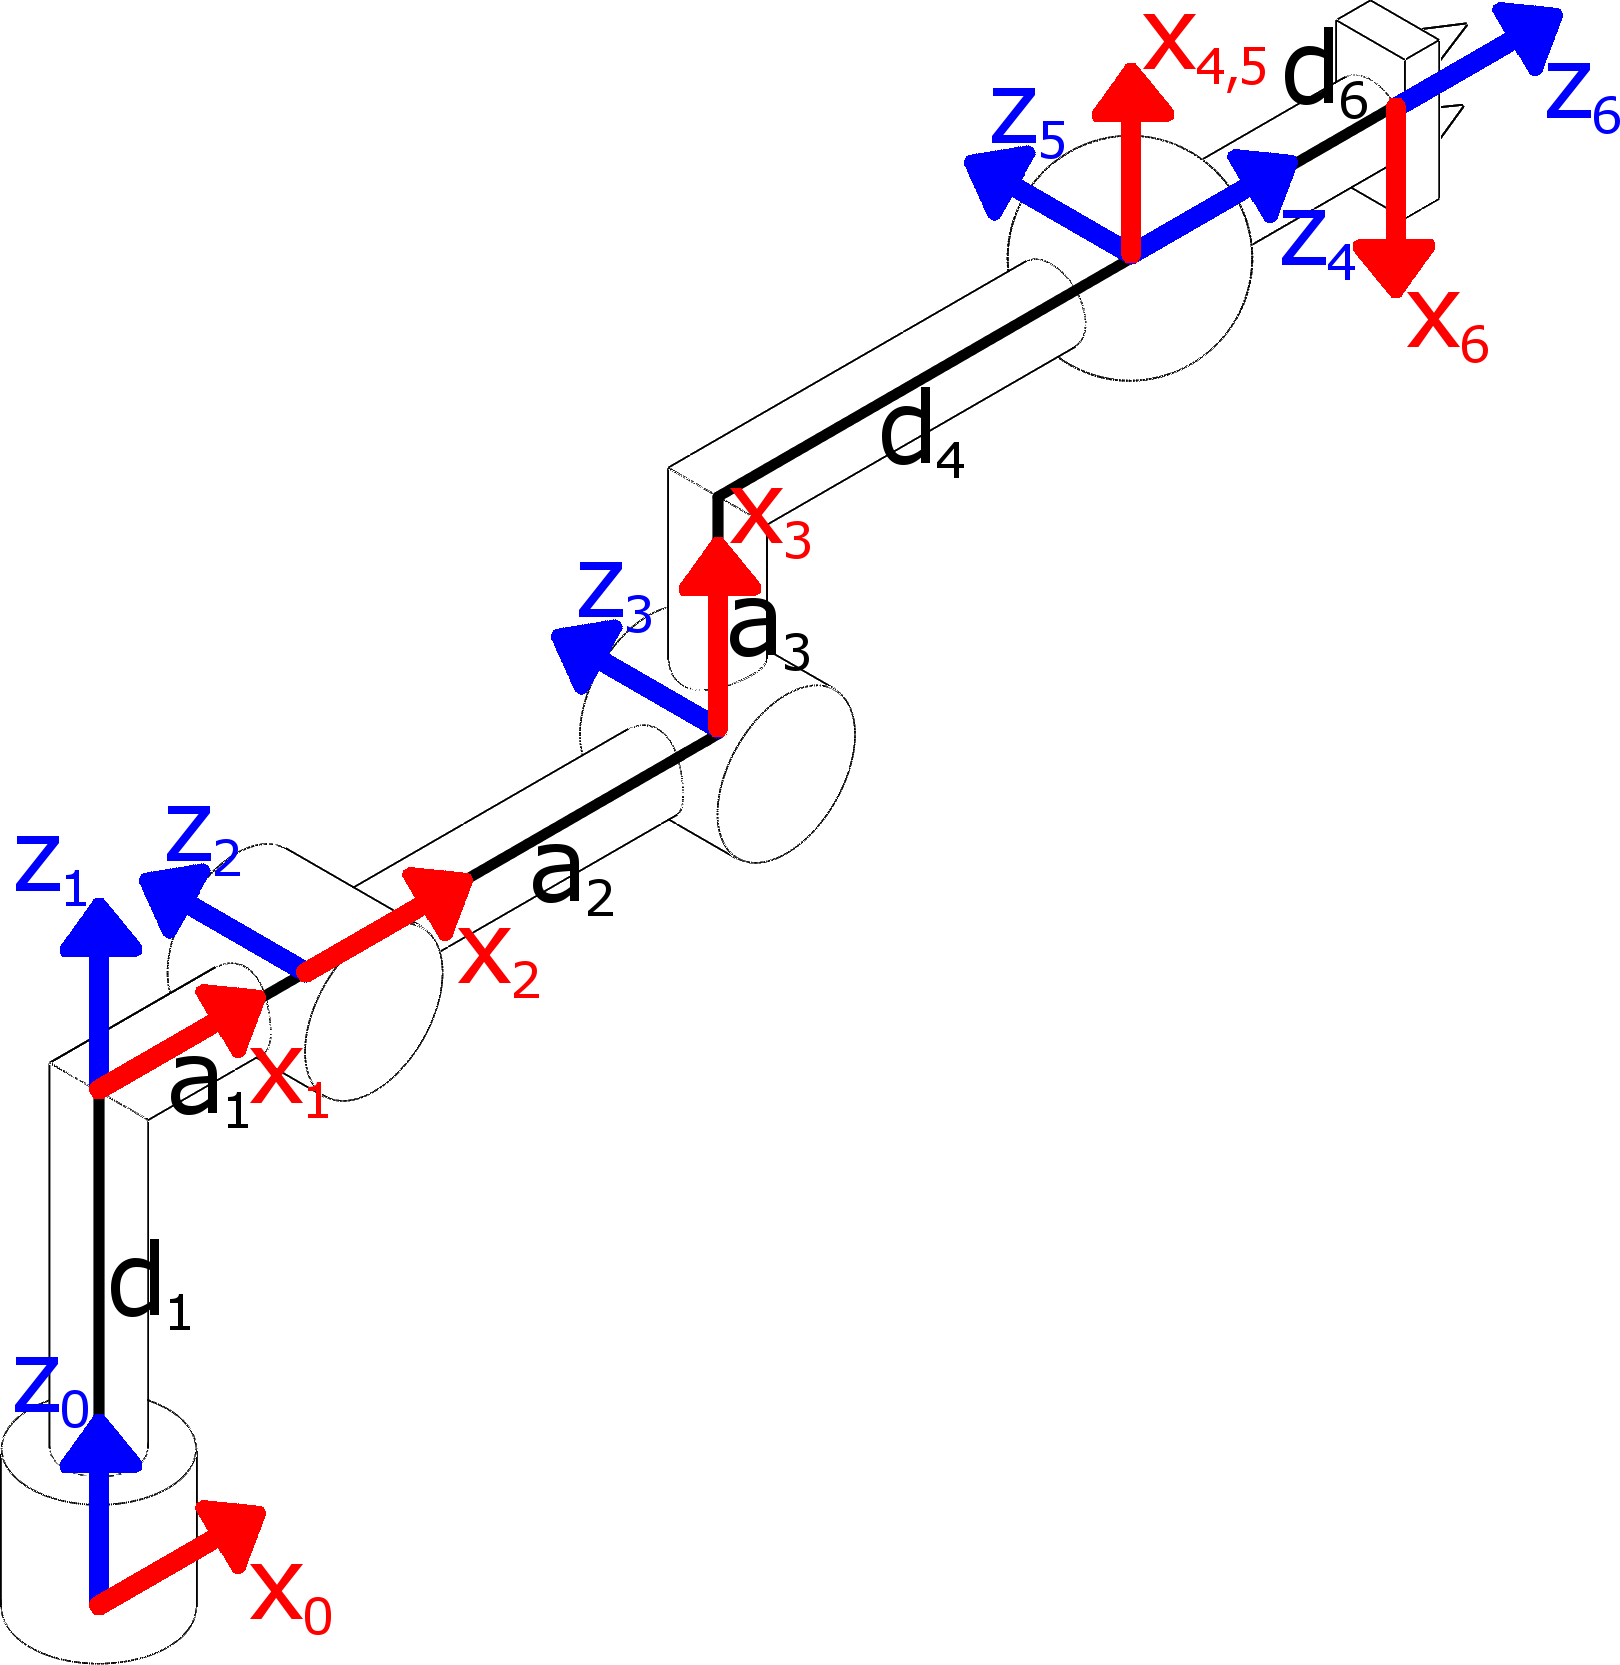
\includegraphics[scale=0.38]{graphics/alex/dh_param.png}}
\end{columns}
\end{frame}


\begin{frame}{Kinematic Model}{Inverse Kinematics}
\begin{itemize}
    \item Joint variables
    \item Position and orientation of end-effector
    \item Application
    \begin{itemize}
        \item Cartesian coordinates
    \end{itemize}
    \item Approach 
    \item Configurations
    \item Solutions
\end{itemize}
\end{frame}

\begin{frame}{Kinematic Model}{Trajectory Planning}
\begin{itemize}
    \item Joint space trajectory
    \item Cartesian space trajectory
    \item Advantages and disadvantages
\end{itemize}
\end{frame}

\begin{frame}{Programming}{Off-line and On-line}
\begin{columns}
\column{0.4\textwidth}
\begin{itemize}
    \item Off-line vs On-line
    \begin{itemize}
        \item Advantages
        \item Disadvantages
    \end{itemize}
    \item \textit{UR5}
    \begin{itemize}
        \item \textit{PolyScope}
        \item \textit{URScript}
    \end{itemize}
\end{itemize}
\column{0.6\textwidth}
\centering{
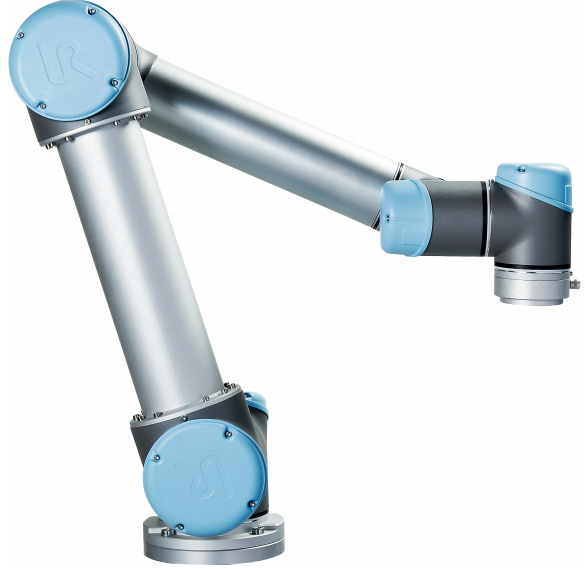
\includegraphics[scale=0.27]{graphics/alex/ur5_design.png}}
\end{columns}
\end{frame}

\begin{frame}{Programming}{RobotStudio}
\begin{columns}
\column{0.5\textwidth}
\begin{itemize}
    \item CAD model
    \item Geometries
    \item Waypoints
    \item Orientation representation
    \item Conversion script
\end{itemize}

\column{0.5\textwidth}
\centering{
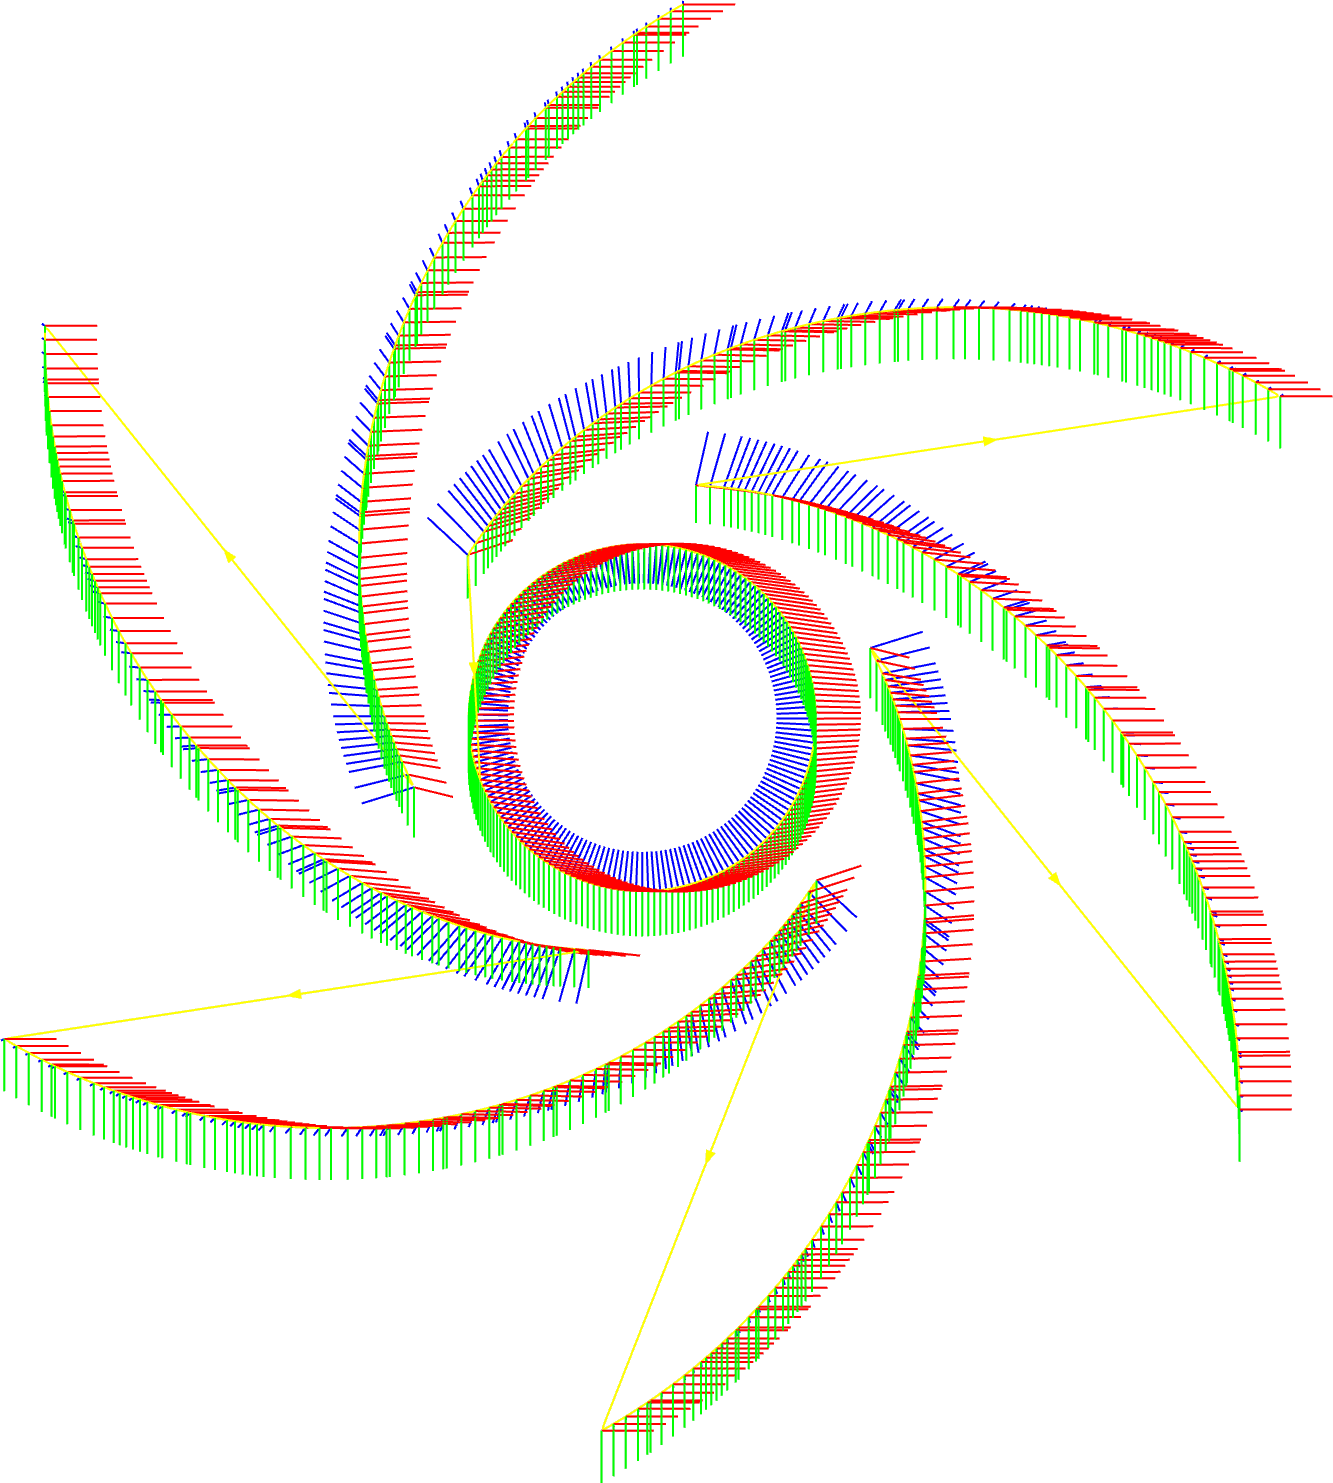
\includegraphics[scale=0.099]{graphics/alex/trajectory_1.png}}
\end{columns}
\end{frame}
\phantomsection
\section{Discussion}
\begin{frame}{Discussion}{Jesper F. Hansen}

\begin{table}[]
    \centering
\begin{tabular}{l l l}
    \hline
    \rowcolor{beamer@barcolor}\textbf{Requirement} & \textbf{Result} \\
    \hline
    Workcell dimensions & Simulated \\
    \rowcolor{beamer@barcolor} Workcell Safety & Simulated \\
    Material flow & Simulated \\
    \rowcolor{beamer@barcolor} Cycle time & Failed \\
    \hline
\end{tabular}
\caption{Results from the simulations}
\end{table}
\begin{itemize}
    \item Inaccuracies in the simulations
    \begin{itemize}
        \item No physical forces included
        \item Point-to-point motion
    \end{itemize}
\end{itemize}
\end{frame}

\begin{frame}{Discussion}{Testing}
\begin{table}[]
    \centering
\begin{tabular}{l l l}
    \hline
    \rowcolor{beamer@barcolor}\textbf{Requirement} & \textbf{Result} \\
    \hline
    Industrial manipulator & Succeeded \\
    \rowcolor{beamer@barcolor}Constant velocity & Failed \\
    Relative distance & Succeeded\\
    \rowcolor{beamer@barcolor}Perpendicular angle & Succeeded\\
    $30.0\degree$ angle & Succeeded \\
    \rowcolor{beamer@barcolor}Deviation & Failed \\
    \hline
\end{tabular}
\caption{Results from the tests}
\end{table}
\begin{itemize}
    \item UR5 vs KUKA KR6 R700 Sixx
    \begin{itemize}
        \item Repeatability
        \item Configuration
        \item Reach
    \end{itemize} 
    \item Laser
    \item CAD model
    \item Script
\end{itemize}
\end{frame}

\section{Conclusion}
\begin{frame}{Conclusion}
"\textit{Therefore, it can be concluded that without further improvements, the} CORPS \textit{is not a feasible solution for implementation in }Grundfos’\textit{ production line.}"
\begin{itemize}
    \item Alternative solutions:
    \begin{itemize}
        \item Turning impeller
        \item Spot weld
    \end{itemize}
\end{itemize}
\end{frame}

\section{Future Work}
\begin{frame}{Future Work}
\begin{itemize}
    \item Sustainability and stakeholders
    \item Simulation
    \item Elimination of inaccuracies
\end{itemize}
\end{frame}

\section{Process Analysis}
\begin{frame}{Process Analysis}{Collaboration}
\begin{itemize}
    \item Group
    \begin{itemize}
        \item Good intent
        \item Misunderstandings
        \item "Two camps"
        \item What could we have done
    \end{itemize}
    \item Supervisors
    \begin{itemize}
        \item Loose contract
        \item Generally satisfied
    \end{itemize}
\end{itemize}
\end{frame}

\begin{frame}{Process Analysis}{Planning}
\begin{itemize}
    \item Timetable
    \item Scrum board
    \item Daily meetings
    \item Laboratory schedule
\end{itemize}
\end{frame}




{\aauwavesbg
\begin{frame}[plain,noframenumbering]
  \finalpage{Feedback, comments and questions}
\end{frame}}
%%%%%%%%%%%%%%%%

\end{document}
